\documentclass[12pt,a4paper]{article}

\usepackage{mystyle} % mit dieser Zeile werden die Pakete in das Dokument eingelesen, das Dokument mystyle.sty muss dazu im directory vorhanden sein

\newcommand{\Title}{The Information Content of VIX Volatility}
%in Comparison to Historic Volatility} 
\newcommand{\Arbeit}{Humboldt Research Project Project}
\newcommand{\Seminar}{Modul 11251 Forschungsprojekt}
\newcommand{\Name}{Sophia Charlotte Gläser}
\newcommand{\MatrikelNummer}{15202284}
\newcommand{\Programme} {Corporate Management and Economics}
\newcommand{\Date}{31.01.2019}
\newcommand{\Semester}{Fall Semester 2018}
\newcommand{\Pruefer}{Prof. Dr. Franziska Peter}
\newcommand{\Chair}{Chair of Empirical Finance and Econometrics}
	
\addbibresource{./bib/bibliography.bib} % das entsprechende File muss ebenfalls im entsprechenden Ordner vorhanden sein


\usepackage{acro}
\DeclareAcronym{BS}{short = BS, long = Black-and-Scholes-Merton Model}
\DeclareAcronym{CBOE}{short = CBOE, long = Chicago Board of Options Exchange}
\DeclareAcronym{SPX}{short = SPX, long = S\&P 500}
\DeclareAcronym{H1}{short = H1, long = Hypothesis 1, class = hypo}
\DeclareAcronym{H2}{short = H2, long = Hypothesis 2, class = hypo}
\DeclareAcronym{H3}{short = H3, long = Hypothesis 3, class = hypo}
\DeclareAcronym{H4}{short = H4, long = Hypothesis 4, class = hypo}
\DeclareAcronym{VIX}{short = VIX, long = Volatility index}

\begin{document}


	\begin{centering}
\Large \textbf{Zeppelin Universität}\\
\Large \Chair \\
\vfill
\LARGE \textbf{\Title} \\
\vfill
\LARGE \Arbeit\\
\vfill
\begin{small}
\begin{doublespace}
\begin{tabbing}
	Student numberrrrrrrr \=\kill
	Name:\>\Name\\
	Student number:\>\MatrikelNummer\\
	Programme:\>\Programme\\
	Term:\>\Semester\\
	Examinor:\>\Pruefer\\
	Due date:\>\Date
	\end{tabbing}
\end{doublespace}
\end{small}
\end{centering}\vspace{1cm}

% Deutsche Version
% \begin{centering}
% \Large \textbf{Zeppelin Universität}\\
% \Large \Chair \\
% \vfill
% \LARGE \textbf{\Title} \\
% \vfill
% \LARGE \Arbeit\\ %Bachelorarbeit
% \Large in \\
% \LARGE \Seminar\\
% \vfill
% \begin{small}
% \begin{doublespace}
%	\begin{tabbing}
%	Immatrikulationsnumerrrrrr \=\kill
%	Bearbeitet von:\>\Name\\
%	Immatrikulationsnummer:\>\MatrikelNummer\\
%	Studiengang:\>\Programme\\
%	Semester:\>\Semester\\
%	Prüfer:\>\Pruefer\\
%	Abgabedatum:\>\Date
%	\end{tabbing}
% \end{doublespace}
% \end{small}
% \end{centering}\vspace{1cm}
	\newpage
	
	\pagenumbering{Roman}
	\tableofcontents
	\listoftables
	\listoffigures
	\printacronyms[exclude-classes=hypo]
	
	\newpage
	
	\pagenumbering{arabic}
	\setcounter{page}{1}
	
	\begin{abstract}
		%!TEX root = ../Main.tex 

This paper investigates the information content of model-free implied volatility for daily realized volatility of the S\&P 500, using the \ac{VIX} from the Chicago Board of Options Exchange and daily volatilities from 2000 to 2017. In contrast to earlier implied volatilities, the VIX is not based on any specific option pricing model. Therefore, it provides a direct test of market efficiency and does not suffer from the joint hypothesis problem. For the statistical analysis the approach from an HAR-RV model as described by \textcite{corsi2009} is used, thus including not only daily, but also weekly and monthly historic volatility in the encompassing regression analysis. The results show, that the \ac{VIX} provides additional information compared to historic volatility, but is not able to subsume all the information contained in the historic volatilities, which partly contradicts previous research. This results are robust to serial correlation and alternative sampling methods. 
	\end{abstract}
	\newpage


	%!TEX root = ../Main.tex

\section{Introduction: The Importance of Volatility Estimation}\label{sec:1Intro}

Financial market volatility is of high interest for the financial sector. Asset return volatility is for example key input to the pricing of financial instruments like derivatives, or to risk measures such as the Value at Risk. Moreover they give information on the risk-return trade-off, which is a central question in portfolio allocation and managerial decision making. \\
As however volatility is not directly observable, it has to be estimated. Seeing its importance, it is not astonishing that during the last years, considerable research has been devoted to the question, how volatility can be estimated and predicted. Two prominent approaches that have been commonly used are time series models, like the ARCH or stochastic volatility models, or implied volatility models, like the \gls{BS} implied volatility models. Whereas time series models rely on historic data, implied volatility models use option price data\footnote{There are, of course, various other methods for volatility estimation and forecasting, such as various nonparametric methods or neural networks based models. However, they shall not be discussed here, for an encompassing overview of volatility estimation and forecasting can be found in \textcite{jiang2003}.}.\\
Out of these two, there has been a growing interest in implied volatility during the the recent years. Since options are contracts giving the holder the right to buy or sell an underlying asset at a specified date in the future, they are said to have a ``forward-looking nature'', meaning that they are supposed to be highly related to the market's expectation about the future volatility of the underlying asset over the remaining life of the option. Therefore, if market agents are rational (meaning that the market uses all available information to form it's expectations about future price movements and volatiltiy) markets are efficient and the model pricing the option is specified correctly, the volatility implied from option prices should be an unbiased and efficient estimator of future realized volatility \parencite{bakanova2010}. Moreover, it should be the best possible forecast possible, given the current information \parencite{christensen2002}. \\
For some time, one popular approach for estimating implied volatility has been the \gls{BS} implied volatility. The \gls{BS} model is an option pricing model, using volatility as an input factor. By using observed option prices as the input and solving for volatility, it is possible to obtain a volatility measure that is widely believed to be ``informationally superior to the historic volatiltiy of the underlying asset'' \parencite[p.1305]{jiang2003}. Early studies found this \gls{BS} implied volatility to be a biased forecast of realized volatility, not containing significantly more information than historic volatility. More recent studies however rejected thesse findings and presented evidence that there is indeed additional information contained in option prices \parencite{jiang2003}. A reason for this discrepancy could be that early studies did not consider several data and methodological problems, such as long enough time series, a possible regime shift around the crash in 1987 and the use of non-overlapping samples \parencite{jiang2003}. \citeauthor{christensen1998} for example took this into account and found that implied volatility outperforms historic volatility. All in all, this new insights provided evidence against the inefficiency of implied volatility.\\
However, even though \gls{BS} implied volatility is found to be the overall more efficient forecast of realized volatility compared to historic volatility, the \gls{BS} implied volatility has some specification problems. Firstly, \gls{BS} implied volatility focuses on at-the-money options. The advantage is, that at-the-money options are the once most actively traded and thus the most liquid ones. However this focus fails to include information contained in other options. Moreover, volatility estimation with the \gls{BS} model includes the same assumptions as are made in the \gls{BS} model itself. Thus, tests based on the \gls{BS} equation are joined tests of market efficiency (as market efficiency has to be assumped to use option prices for volatility estimation, as mentioned above) and the \gls{BS} model, and therefore suffer from model misspecification errors \parencite{jiang2003}. \\
That is why during the last years, implied volatility indexes which are not based on a pricing assumption have gained popularity. One of these model-free implied volatility indexes is the VIX from \gls{CBOE}.






	%!TEX root = ../Main.tex

\section{Selected Estimation and Modelling Procuedures for Volatility}\label{sec:2Models}
As mentioned in \ref{sec:1Intro}, volatility can not be directly observed and thus as to be estimated. This section briefly presents a concept for estimating realized volatility, which is important when it comes to modelling of this volatility. In the following, one example for such a model very well capturing the the stylized facts observed with financial data is presented. 

\subsection{Estimating and Modeling Volatility using Historic Volatility}\label{sec:22Historic}
%
\subsubsection{Estimating Realized Volatility}\label{sec:221RV}
% WHAT IS VOLA%
By definition ``volatility seeks to capture the strength of the (unexpected) return variation over a given period of time'' \parencite[p.7]{andersen2001}. As terminology is not consistent in previous research, return variance is simply the second moment distribution characteristic, and return volatility is the standard deviations, which is the square root of the return variance. \\
However, with volatility being a latent variable, there are multiple concepts for volatility. According to \citeauthor{andersen2001} they can be grouped in (i) the \emph{notional volatility} corresponding to the ex-post sample-path return variability over a fixed time interval, (ii) the ex-ante \emph{expected volatility} over a fixed time interval or the (iii) the \emph{instantaneous volatility} corresponding to the strength of the volatility process at a point in time. Fur the purpose of this paper, which aims at measuring the information content of model-free implied volatility, an estimate for the  notional ex-post sample-path return variability is needed. \\
Volatility measures usually represent the average volatility over a discrete time, as a continuous record of price data is not available, and even for very liquid markets, price data are distorted by micro-structure effects. It can however be shown, that under some assumptions the sum of squared high-frequency returns is a consistent estimator for the return variance. This results mainly builds on the work of \parencite{andersen2001} and will only be briefly introduced here.\\
% REALIZED VARIANCE %
To begin with, it should be assumed that we have a continuous-time no-arbitrage setting. As return volatility aims to capture the strength of the unexpected return variation as defined above, one needs to define the component of a price change as opposed to an expected price movement.\textcite{andersen2001} show, that under certain assumptions the instantaneous return process can be decomposed into an expected return component, and a martingale innovation (in the discrete time setting this decomposition is more complex, for this paper it shall only be relevant that the martingale part is still the dominant contribution to the return variation over short intervals). Furthermore \textcite{andersen2001} show, that the cumulative sample path variability of this martingale component can be represented by a quadratic variation process. To be precise, they define ex-post measured \emph{notional variance} is the increment to the quadratic variation for the return series. Moreover they show, that this notional variance can be consistently estimated using high-frequency returns or a large sample of returns, with the \emph{realized variance}, defined as:
\begin{align}\label{eq:RV-andersen}
v^2(t,h;n) = \sum_{i=1}^{n} r(t-h+(i/n) \times h,h/n)^2
\end{align}
over any fixed $[t-h,t], 0 < h$ time interval (Their proposition 5).\\
So in summary, the increment to the quadratic return variation which is the past variance, can be consistently and well approximated through the accumulation of high-frequency squared returns. Taking the square root of this realized variance, the \emph{realized volatility} is obtained


\subsubsection{Modelling Volatility - HAR-RV Model}\label{sec:222HAR-RV}
Having introduced the concept of measuring realized volatility, there are multiple models that try to model the volatility process. Although volatility is not directly observable, it has some characteristics that are commonly observed and can be used to build volatility models. \\
% STLYZED FACTS%
These commonly observe stylized facts include for example high excess kurtosis for daily return series, and clustering of return variability, meaning that periods of large volatility seem to be followed by high volatility, and periods of low volatility seem to be followed by low volatility \parencite{tsay2005}. Moreover the autocorrelations of the square and absolute returns show a very strong persistence over long time periods. If return distributions with regard to different time horizons are observed, they show not only the fat tails mentioned above, but also tail-crossover, meaning that the shape depends on the time scale. As the time scale increases, the return distribution slowly converge to the normal distribution, however very slowly. Moroever, financial data show evidence of scaling and multi-scaling \textcite{corsi2009}. \\
% INTRO TO HAR-RV MODEL %
There are various modelling approaches for volatility. This paper will refer to the HAR-RV model, based on \textcite{corsi2009}. The model assumes, that prices follow the standard continuous time process , represented by the stochastic differential equation
\begin{align}\label{eq:return-process-corsi}
dp(t) = \mu(t)dt + \sigma(t)dW(t), \ 0 \leq t \leq T
\end{align}
where $p(t)$ is the logarithm of the instantaneous price, $\mu$ is a finite variation stochastic process, $W(s)$ standard Brownian motion and $\sigma$ a stochastic process independent of $W(s)$. For this process, the variance is the \emph{integrated variance}, which is integral of the instantaneous variance over the one-day interval
\begin{align}
IV_{t}^{(d)} =  \int_{t-1d}^{t} \sigma^{2}(w)dw, 
\end{align}
and the corresponding volatility it's square root: $\sigma = \sqrt{IV_{t}^{(d)}}$.
\textcite{andersen2001} show, that instead of the abstract martingale representation of the return decomposition that was described in \ref{sec:221RV}, the continuous sample paths can also be represented using stochastic differential equations, as it is done here. Then the integrated variance equals the notional volatility, and can equally be estimated using the sum of squared returns. Thus, the HAR-RV model uses the following approximation for realized volatility over the one day interval, which shall also be used in this paper:
\begin{align}
RV_{t}^{(d)} = \sqrt{\sum_{j=0}^{M-1} r^{2}_t-j \times \Delta}
\end{align}
with $\Delta = 1d/M$ being the sampling frequency and $r^{2}_t-j \times \Delta$ defined as the continuously compounded $\Delta$-frequency returns. \\
% HETEROGENEOUS MARKET HYPOTHESIS %
The idea behind the HAR-RV model is closely connected to the \emph{Heterogeneous Market Hypothesis}, described by \textcite{mueller1993}, which describes the presence of heterogeneity across market participants. This view of financial markets grounds on the fractal model, introduced and applied to financial markets by \textcite{mandelbrot1963}. The approach of this model is to analyse (time series) objects on different time scales and compare the obtained results. The argument for using this approach is, that conventional time series analysis focusing on regularly spaced observations does not capture the real nature of the raw data, as the usual time choice for recording observations (e.g. a day) is arbitrary. Thus for example a process explaining monthly price changes could not be applied to daily data and vice versa. Using this fractal approach and empirical finding of volatility characteristics gave rise to the heterogeneous market hypothesis. This hypothesis assumes that the market gives rise to heterogeneous trading behaviours as different market participants or components have different time horizons for their trading goals and for their consideration of past events. The time span has on the one side the high-frequency dealers such as market makers, in the middle some medium term dealers and on the other side the low-frequency dealers, such as central banks or commercial organizations. Driven by this components, ''the market is heterogeneous with a ''fractal`` structure of the participants' time horizon`` \parencite[p.12]{mueller1993}. This hypothesis is based on the observations, that the decline of the return autocorrelation function is not exponential, as suggested for example by lower-order GARCH or ARCH models, but rather hyperbolic. Assuming that each of the distinct components has an exponential decline with different time horizons, in sum comes close to a hyperbolic decline. Moreover, if market participants were homogeneous, volatility should be negatively correlated with market activity, as the price should converge to the ``real value''. However, they are positively correlated, which might be explained by the fact that actors react and execute in different market situations \parencite{mueller1993}. Other than to time scale, the heterogeneous market hypothesis can be applied to geographical location, degrees of risk aversion, institutional constraints or transactions costs. However, as in \textcite{corsi2009} for this paper the time aspect should be relevant.\\
% EMPIRICAL JUSTIFICATION OF THE HAR-RV MODEL %
\textcite{corsi2009} adds to the observations of \textcite{mueller1993}, that volatility has an asymmetric behaviour of influence, meaning that volatility over longer time periods has a stronger influence on volatility observed over short periods than conversely. The pattern that emerges from this is a volatility cascade pattern from low to high frequencies. To formalize the model the \emph{latent partial volatility} $\tilde{\sigma}_{t}^{(.)}$ is defined as the volatility generated by a certain market component. To account for short-term, medium-term and long-term traders, the time horizons of one day (1$d$), one week (1$w$) and one month (1$m$) are considered, and denoted by $\tilde{\sigma}_{t}^{(d)}$, $\tilde{\sigma}_{t}^{(m)}$ and $\tilde{\sigma}_{t}^{(w)}$. In the model, each of this volatility components corresponds to a market participant, that forms the expectation for the volatility of one period ahead based on both the observation of the current realized volatility according to the own time frame, and on the expectation of the one horizon longer volatility. For example for the market participant with a daily horizon, the latent volatility would be
\begin{align*}
\tilde{\sigma}_{t+1d}^{d} = c^{d} + \Phi^{(d)} RV_{t}^{(d)} + \gamma^{(d)} E_{t}[\tilde{\sigma}_{t+1w}^{(w)}] + \tilde{w}_{t+1d}^{(d)}
\end{align*}, 
where $\tilde{w}_{t+1d}^{(d)}$ is the return innovation. Substitution the latent volatilities of the different horizons and defining the latent volatility as the daily integrated volatility ($\tilde{\sigma}_{t}^{(d)})$, the cascade model can be written as
\begin{align}\label{eq:cascade-model}
\sigma_{t+1d}^{(d)} = c + \beta^{d} RV_{t}^{(d)} + \beta^{(w)} RV_{t}^{(w)} + \beta^{(m)} RV_{t}^{(m)} + \tilde{w}_{t+1d}^{(d)},
\end{align}
Observing the volatility data ex-post, $\sigma_{t+1d}^{(d)}$ can be written as the realized volatility, a functional form for time series representation can be written as:
\begin{align}\label{eq:time-series-model}
RV_{t+1d}^{(d)} = c + \beta^{d} RV_{t}^{(d)} + \beta^{(w)} RV_{t}^{(w)} + \beta^{(m)} RV_{t}^{(m)} + w_{t+1d} ,
\end{align}
where $w_{t+1d}$ includes the innovation component and the measurement and estimation error. In the time series model, the realized volatility for the weekly and monthly aggregated periods are simply the rolling average over the respective periods.
% SIMULATION RESULTS WITH HAR-RV MODEL %
Using simulated return data, \textcite{corsi2009} shows, that the HAR-RV simulated returns and volatility reproduce the stylized facts mentioned above very well. The data has not only the excess of kurtosis , but also the tail cross-over, meaning that the fat tails get thinner as the aggregation level increases. Concerning the volatility memory, the simulated data is also able to reproduce the long memory of the empirical data. Moreover, using OLS, in-sample and out-of-sample forecast, \textcite{corsi2009} shows, that the past volatility components all have significant information content for one day ahead realized volatility and good forecasting performance.

\subsection{Estimating Volatility Using Option Price Data - Implied Volatility}
\subsubsection{The General Idea and Evolution of Implied Volatility}
% INTRO IMPLIED VOLA, EXAMPLES: BS %
Apart from using historic data for volatility modelling, another approach is to use the forward-looking nature of options data to augment the information set. This approach can be termed \emph{implied volatility}. The intuition behind implied volatility is, that option prices can be seen as reflecting market participants' expectations of the future movements of the underlying asset. Assuming that the marked is efficient, as described by \textcite{fama1970}, and that the asset pricing model is correct, the implied volatility derived from this model should not only subsume all information contained in the models using historic volatility, but also be a more efficient forecast of future volatility \parencite{jiang2003}. \\
One example for implied volatility is the \emph{\ac{BS} implied volatility}, building on the \ac{BS} asset pricing model as presented by \textcite{black1973}, which uses volatility as one input for pricing options. Having the option prices available on the market, it is possible to extract a value for the expected volatility by inverting the theoretical asset pricing model. \\
% LITERATURE REVIEW (BS) IMPLIED VOLA %
Many studies examined the information content of \ac{BS} implied volatility and it's forecasting ability for future volatility. Earlier studies (for example \textcite{canina1993} find that implied volatility contains little additional information content compared to historical volatility and has no forecasting ability. In contrast, other studies  support the evidence of implied volatility subsuming the information from historic volatility. These are for example \textcite{day1992}, \textcite{lamoureux1993} or \textcite{jorion1995}.\\
With previous research leading ambiguous results, more recent research made several methodological and data corrections and found evidence supporting the hypothesis that implied volatility has predictive power for future volatility. These corrections included using longer time series, adapting high-frequency asset returns or using non-overlapping samples \parencite{jiang2003}. \textcite{christensen2001} found that under certain of these measurement errors (such as overlapping samples) statistical tests are no longer meaningful. Correcting for this meassurement errors results in support for the hypothesis, that implied volatility subsumes all information contained in historic volatility. All in all, this insights provide a convincing argument why early studies found the forecast of implied volatility to be inefficient \parencite{jiang2003}. \\
% FAILURES OF BS IMPLIED VOLA %
However, even though recent evidence is in support of \ac{BS} implied volatility, there are several disadvantages of using the implied volatility with an asset pricing model. One disadvantage is, that the \ac{BS} implied volatility relies mostly on information from at-the-money options, which are generally the most actively traded ones. This however fails to incorporate information contained in other options. Moreover and more importantly, testing for the \ac{BS} implied volatility always means testing market efficiency and the \ac{BS} model jointly. Assumptions of the \ac{BS} model include constant volatility, no transaction costs or taxes, no dividend before option maturity, no arbitrage, continuous trading, constant risk-free interest rate, divisible securities and no short sell \parencite{poon2003}. As it is not possible in this setting to test for market efficiency or the pricing assumptions separately, this tests are subject to model misspecification errors \parencite{jiang2003}. This is why an implied volatility that does not rely on an asset pricing model was introduced. 


\subsubsection{Model-Free Implied Volatility and the VIX}\label{sec:223VIX}
% INTRO MODEL-FREE IMPLIED VOLA %
The idea of model free implied volatility was introduced by \textcite{britten2000} who show that the risk-neutral realized volatiltiy can be derived from a set of options with matching expiration, thus extendending the approach of \textcite{derman1994} \textcite{dupire1994}, \textcite{dupire1997} and \textcite{rubinstein1994} on implied distributions. Contrary to \ac{BS} implied volatility, no assumptions are made concerning the pricing process. Instead, a complete set of option prices is taken as given and as much information as possible is extracted about the underyling price process \parencite{britten2000}. \\
% BRITTEN PAPER %
\textcite{britten2000} show in an approach resembling a binomial tree, that the probability of the stock price reaching any particular level and of a price move is determined by the initial set of option prices. Moreover they show that the risk-neutral expected sum of squared returns between to dates is given from the set of options expiring on these to dates (their proposition 2). This formula does not use any specific option pricing model to derive implied volatility and is only based on no-arbitrage conditions, therefore it solves the joint-hypothesis problem and test directly for market efficiency \parencite{jiang2003}.  \\
% LITERATURE REVIEW MODEL-FREE IMPLIED VOLA %
Several paper used this result and compared the informational efficiency of model-free implied, \ac{BS} and historic volatility. One paper that examines the information content of model-free implied volatility is \textcite{jiang2003}. They use the approach of \textcite{britten2000}, extend the formula to asset price processes with jumps and test the informational efficiency of this model-free implied volatility in comparison to both \ac{BS} implied and historic volatility, using both univariate and encompassing regression analysis. Using option data from the S\&P 500 for the model-free implied volatility calculation and 5-min returns to calculate daily realized volatility, they examine monthly non-overlapping samples of a 6-year sample period between June 1988 and December 1994. Their findings are, that the model-free implied volatility subsumes all the information contained in the \ac{BS} implied volatility and past realized volatility. Another example is the paper of \textcite{bakanova2010}. With daily data from oil futures between November 1986 and December 2006, they evaluate the information content of model-free implied volatility in comparison to historic volatility using a monthly frequency. 
Using regression analysis, they come to the result that implied volatility subsumes the information contained in historical volatility. In contrast to these results is for example \textcite{taylor2010}. With individual stock data from 149 U.S. firms between January 1996 and December 1999, they find that for a one-day-ahead estimation, historic volatility outperforms model-free implied volatility- When however extending the prediction horizon, the option implied volatility is more informative. \\
% VIX INTRODUCTION %
One of the first implemented implied volatility index was the \ac{VIX} from the \ac{CBOE}. It is computed each trading day on a real-time basis, with data available dating back to January 1986. It's introduction in 1993 had the intention to provide both a benchmark for market volatility in the short term, and a volatility index on which futures and options could be written and traded. At this time the \ac{VIX} was based on the \ac{BS} option pricing model using S\&P 100 options, as they where the most actively traded in the U.S. \parencite{whaley1995}. In 2003 the \ac{VIX} adopted to the changes that took place in the options market. First, the S\&p 500 option market superseded the S\&P 100 options market as the most actively traded option market in the U.S., thus following 2003 the \ac{VIX} was based on the S\&P 500 options. Secondly, option index trading behavior changed. Whereas in the 1990s both call and put index options where equally important, over the years both out-of-the money and at-the-money puts gained popularity as they were bought by portfolio insurers. Thus the \ac{VIX} also started to include out-of-the money options in it's calculation, bringing another advantage compared to \ac{BS} implied volatility \parencite{whaley2008}. Finally, the \ac{VIX} calculation changed in 2003, adopting to the model-free implied volatility approach, which was in 2003 widely used by financial theorists, risk managers, and volatility traders alike \parencite{exchange2009}.\\
% VIX CALCULATION %
The \ac{VIX} is constructed in the way that it eliminates mis-specification and ``smile'' effects thus making it an accurate measurement of implied volatility \parencite{blair2001}. The formula for calculation is
\begin{align}\label{eq: VIX}
VIX = \sqrt{\frac{2}{T} \sum_{i} \frac{\Delta K_{i}}{K_{i}^{2}} e^{RT} Q(K_{i}) - \frac{1}{T} (\frac{F}{K_{0}} - 1)^{2}} \times 100
\end{align}
with $T$ being time to expiration , $F$ the forward index level, $K_{0}$ the first strike below the forward index level, $K_{i}$ the strike of the $i^{th}$ out-of-the-money option, $\Delta K_{i}$ the interval between the strike prices, $R$ the risk-free rate and $Q(K_{i})$ the midpoint of bid-ask spread for each option with strike $K_{i}$. For the calculation first the options used for calculation are selected. The \ac{VIX} always uses near- and next-term put and call options, with more than 23 and less than 37 days to expiration. Each week, the options used for calculation roll over to new maturities, thus long-term options become next-term options, and in the following week fall out of the sample. Thus the \ac{VIX} will always reflect an interpolation of the volatility between these two option maturities, using the midpoint bid-ask price as the transaction price are subject to bid-ask bounde \parencite{poon2003}. After the selection of the options for the calculation, the volatility for both the near- and next-term options is calculated. Out of this two volatility, the 30-day-weighted average is calculated, so that the \ac{VIX} gives information about the expected volatiltiy over the next 30 days. \parencite{exchange2009}. 


%  This requires the decomposition of the return process in an expected and an innovation component. 

%(\textcite{canina1993} for example use only a 4-year range of data from 1983 to 1987)

%Moreover, they show that realized variance can serve as an an unbiased estimator of the expected variance.\\

%plus estimation error ($\sigma_{t+1d}^{(d)} = RV_{t+1d}^{(d)} + w_{a+1d}^{(d)}$),

%= \tilde{w}_{1+d}^{(d)} - w_{1+d}^{(d)}$, thus

% For a very comprehensive overview of the volatility research as was state of the art in 2003, please see \textcite{poon2003}.

%This leads them to their proposition 1, that the expectation of the squared return, conditional on stock price and time, is determined by the initial option prices. Moreover, as this proposition one only infers a one-period forecast conditional on a stock price level, they propose a forecast over any multiperiod interval without conditioning, by showing that the risk-neutral expected sum of squared returns between to dates is given from the set of options expiring on these to dates (their proposition 2).

% conducted forecasts using the model free implied volatility or extended the concept. Here, particularly the paper measuring the information content are relevant.

%, which is critical to the usefullness of the VIX or any other implied volatiltiy index.

%\textcolor{gray} {Sometimes the VIX is called \emph{investor fear gauge}, however it is important to notice that it measures, not causes market volatility. It is true, that using regression analysis \textcite{whaley2008} found, that the rate of change in the VIX and S\&P 500 is asymmetric, with the VIX reacting higher to a drop in the S\&P 500 than its rise, which could be interpreted as a higher fear in the downside then excitement in an up-move. Nevertheless, this correlation must not express causality \parencite{whaley2008}.} % make this the part about literature concerning volatility measurement
	%%!TEX root = ../Main.tex

\section{Empirical Results on the Information Content of Model-Free Implied Volatility and Hypothesis}\label{sec:3Literature}

% removed









 % suggestion Fr.Peter - take this part about literature concerning volatility forecast out
	%!TEX root = ../Main.tex

\section{Methodology and Data}
\subsection{Methodology: Linear Regression and HAR-RV model}
\begin{itemize}\itemsep0pt
\item Reg1: without VIX
\begin{itemize}\itemsep0pt
\item Reg1a: regress realized volatility on historic volatility using simple linear regression
\item Reg1b: regress realized volatility on historic volatility using HAR-RV model
\end{itemize}
\item Reg2: with VIX
\begin{itemize}
\item Reg2b: regress realized volatility on historic volatility using simple linear regression
\item Reg2b: regress realized volatility on historic volatility using HAR-RV model
\end{itemize}
\end{itemize}
%
\begin{flalign}
&\sigma_{t,x}^{RV} = \alpha_{x,t} + \beta_{x,t}^{HV} \sigma_{x,t}^{HV}\\
&\sigma_{x,t}^{RV} = \alpha_{x,t} + \beta_{x,t}^{HV,d} \sigma_{x,t}^{HV,d} + \beta_{x,t}^{HV,w} \sigma_{x,t}^{HV,w} + \beta_{x,t}^{HV,m} \sigma_{x,t}^{HV,m}\\
&\sigma_{x,t}^{RV} = \alpha_{x,t} + \beta_{x,t}^{HV} \sigma_{x,t}^{HV} + \beta_{x,t}^{VIX} + \sigma^{VIX}_{x,t}\\
&\sigma_{x,t}^{RV} = \alpha_{x,t} + \beta_{x,t}^{HV,d} \sigma_{x,t}^{HV,d} + \beta_{x,t}^{HV,w} \sigma_{x,t}^{HV,w} + \beta_{x,t}^{HV,m} \sigma_{x,t}^{HV,m} + \beta_{x,t}^{VIX} + \sigma^{VIX}_{x,t}
\end{flalign}

\subsection{Data and Calculation of Input Factors}

Graphics


\begin{figure}[!htbp]
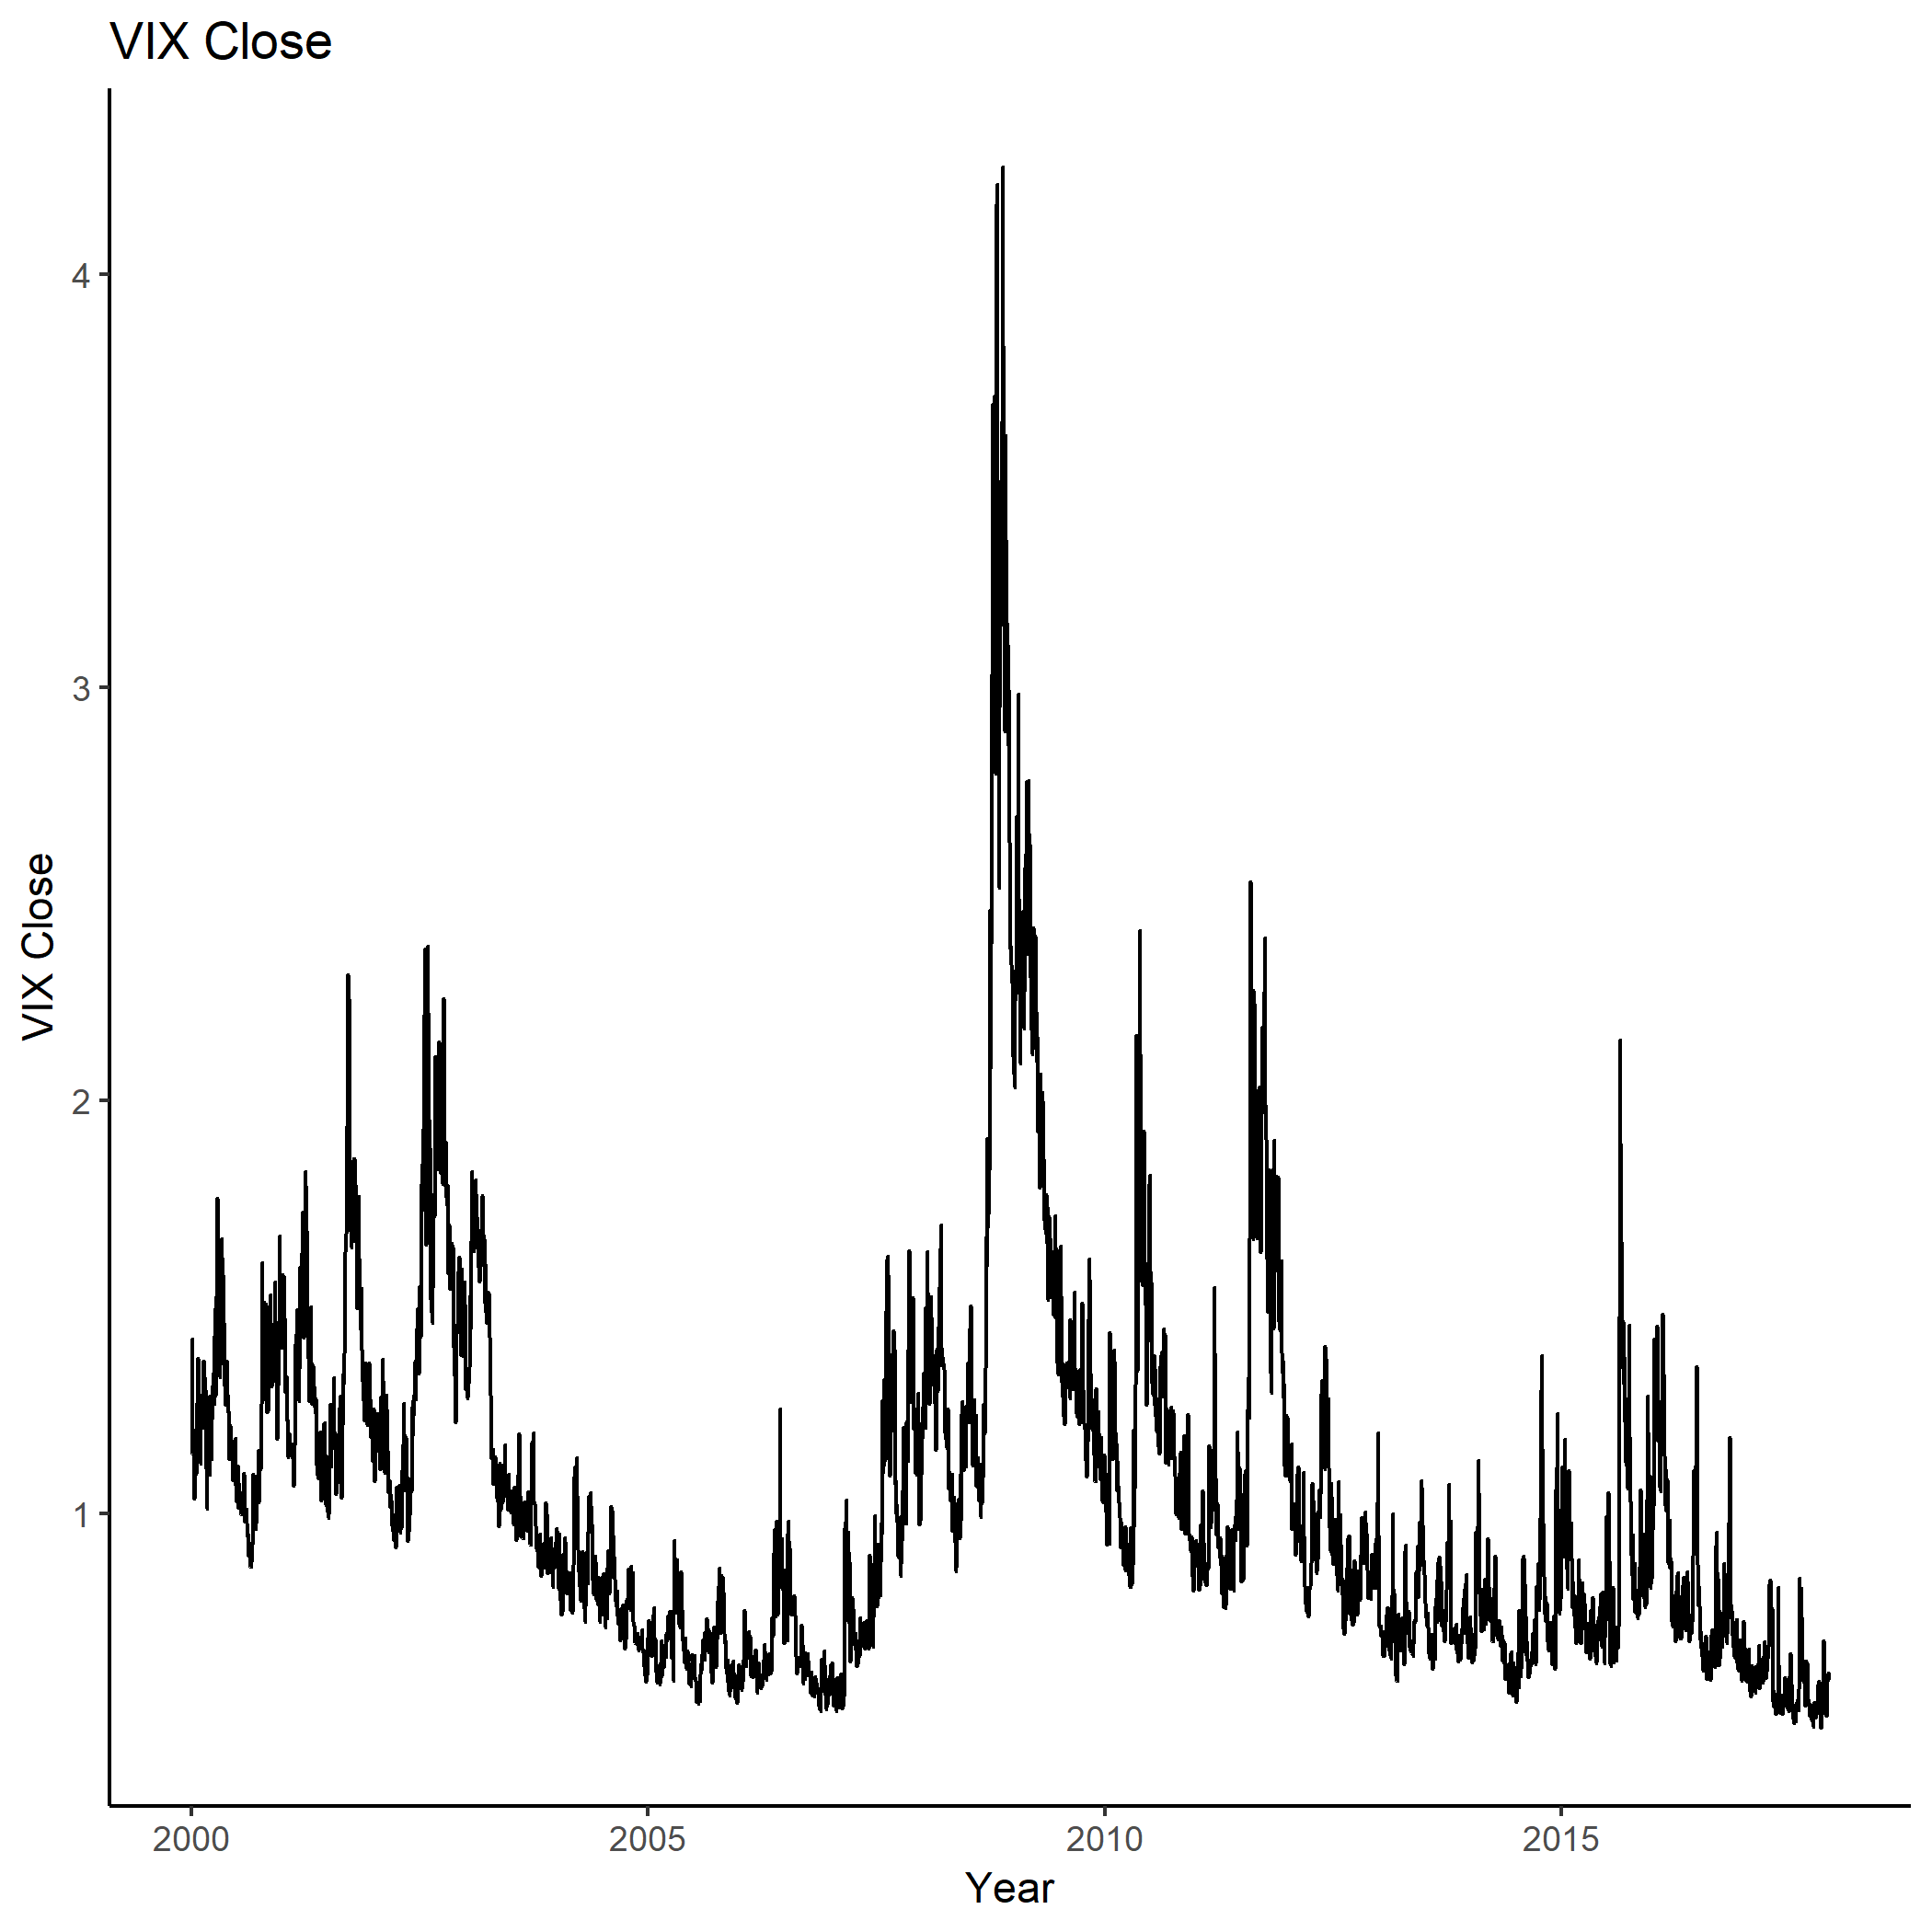
\includegraphics[width=16cm, height=8cm]{pictures/vix.png}
\end{figure}
%
\begin{figure}[!htbp]
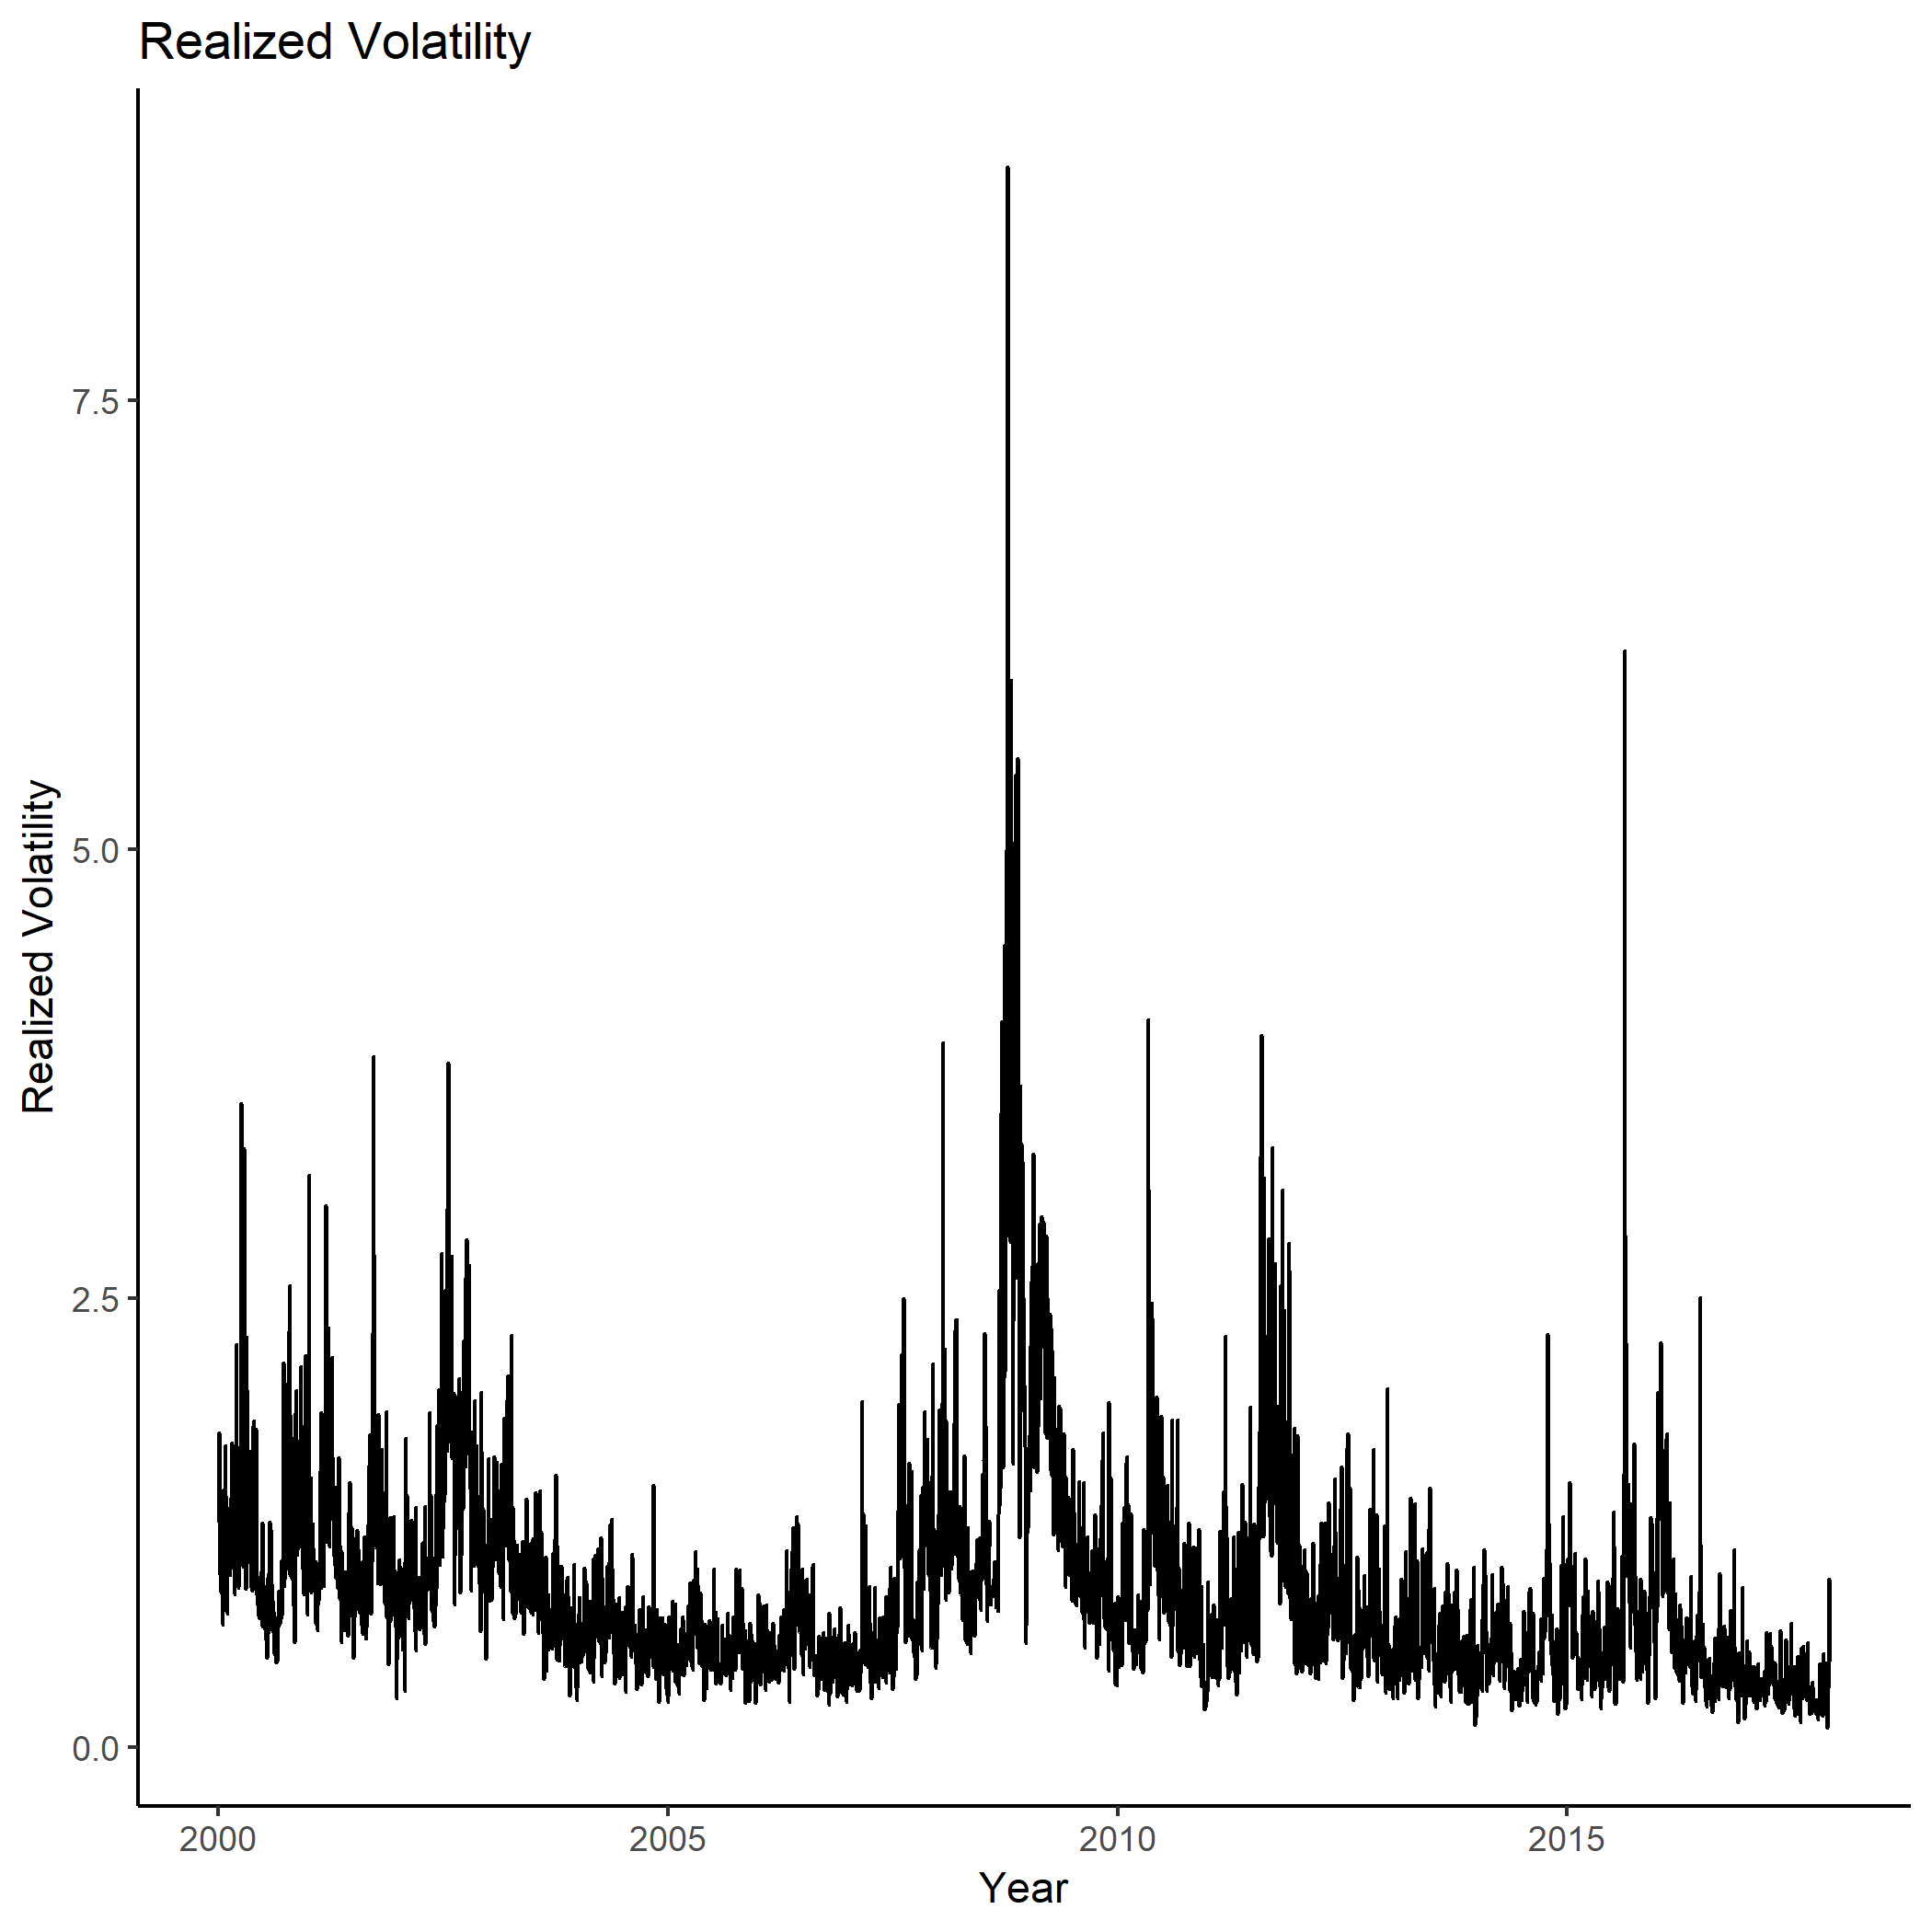
\includegraphics[width=16cm, height=8cm]{pictures/vol.png}
\end{figure}
%
\begin{figure}[!htbp]
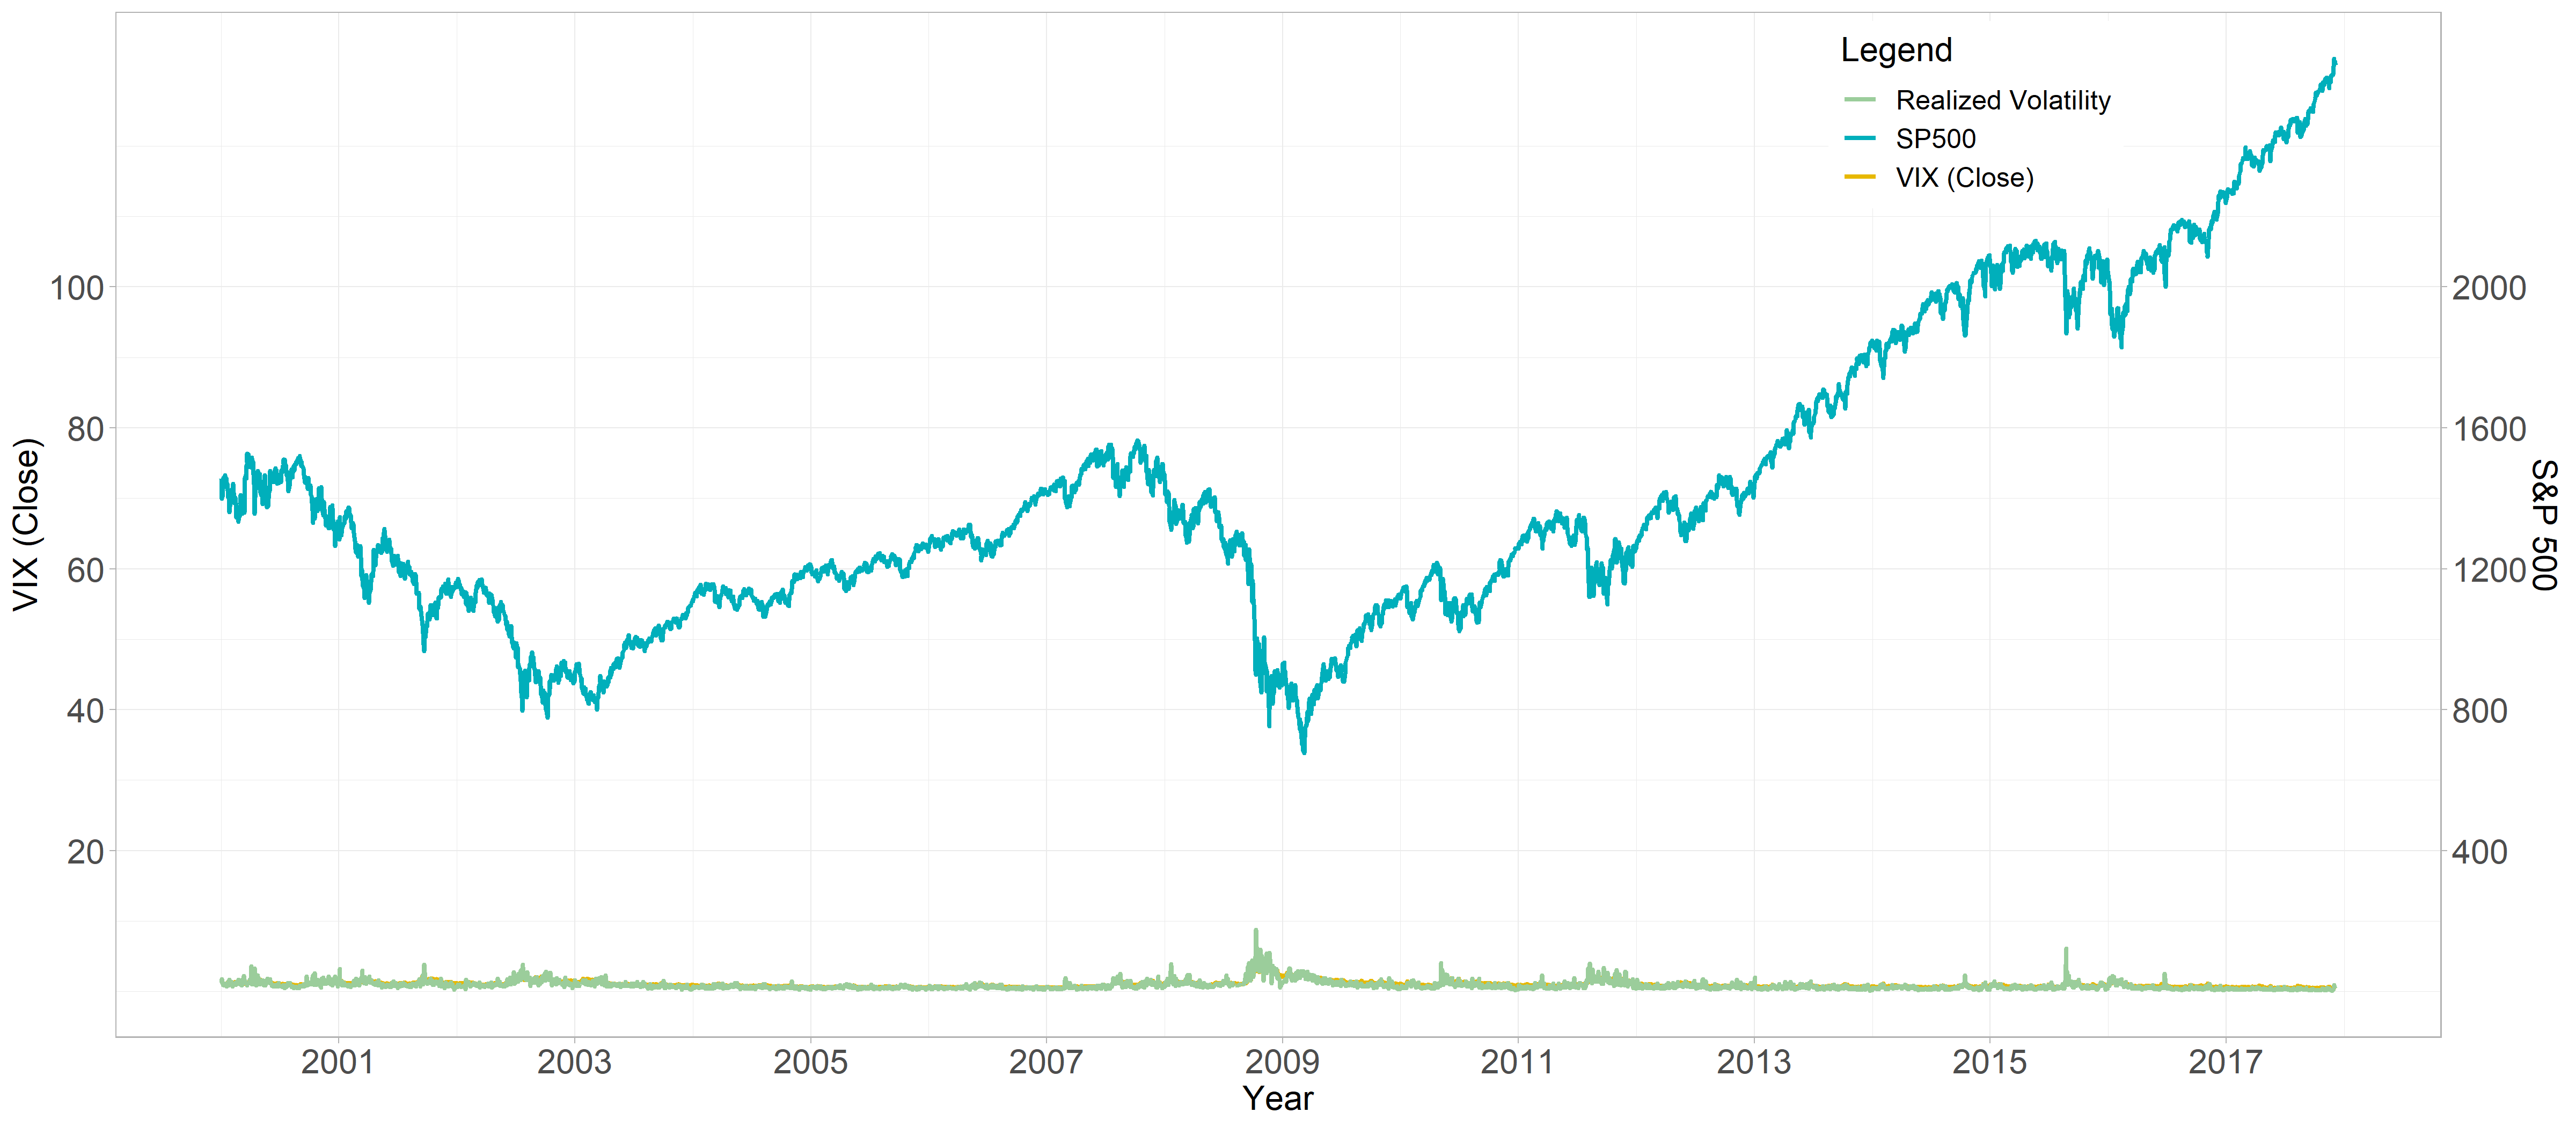
\includegraphics[width=16cm, height=8cm]{pictures/SPandVolandViX.png}
\end{figure}

Measure for daily return variability should be realized volatility, as \citeauthor{andersen2001} suggest, that under suitable conditions it provides an unbiased estimator of the return volatility. 


\begin{itemize}\itemsep0pt
\item S\&P 500 index data on daily basis
\item sampling period: 2000 - 2018
\item realized volatility: daily realized volatility of S\&P 500, calculated using 5 minute returns, retrieved from \citeauthor{heber2009}
\item model-free implied volatility: VIX index data
\item historic volatility: lagged realized volatility, for HAR-RV model use the average over the time period used to forecast
\end{itemize}

	%!TEX root = ../Main.tex

\section{Results}\label{sec:5Results}

This section presents the estimation results. The first subsection reports the results obtained with the regression analysis described in section \ref{sec:42Method}. The second subsection provides the results of the robustness checks conducted. 

\subsection{Regression Analysis Results}\label{sec:51Regression}
In the following, the regression results are presented. The regression outputs can be found in table \ref{tab:newey2} for the logarithmic regression and \ref{tab:newey1} for the level regression, in the appendix. To make it easier to overview the results, only one regression table was included in this section. The logarithmic table is displayed, since as discussed in \ref{sec:41Data} it should be better specified, which is confirmed by it having a lower AIC than the level specification.\\
Firstly, if the VIX contains information about future realized volatility, the slope of the VIX in \ref{eq:Reg1b} and \ref{eq:Reg2b} should be positive and significantly different from zero. The $H_{0}: \beta^{VIX} = 0$ can be rejected for both the level and the logarithmic regression specification, which implies that the VIX contains significant information for future volatility. Thus the \textbf{\ac{H1}} can be confirmed.\\
Secondly, if the VIX has more explanatory value than the historic volatilities, the adjusted $R^{2}$ in the second regression with the \ac{VIX} (\ref{eq:Reg2a} and \ref{eq:Reg2b}) should be larger than in the first regression with the historic volatilities (\ref{eq:Reg1a} and \ref{eq:Reg1b}). This not true for both the level and the logarithmic specification. Even though the $R^{2}$'s are close, they are slightly larger in the first regression ($0.726$) than in the second ($0.693$). Thus, the \textbf{\ac{H2}} can not be confirmed.\\
Thirdly, if the VIX adds explanatory value to the historic volatilities, the adjusted $R^{2}$ in the third regression (\ref{eq:Reg3a} and \ref{eq:Reg3b}) with the VIX included should be larger than in the first regression, containing only the historic volatilities. This is true for both specifications, in alignment with \textbf{\ac{H3}}.\\
Finally, if the VIX subsumes all information contained in the historic volatilities, the historic volatilities should not be significantly different from zero, contrary to the VIX. Thus the $H_{0}: \beta^{d} = \beta^{w} = \beta^{m} = 0 \ and \ \beta^{VIX} = 1$ should not be rejected. The F-test results however provide the result, that the $H_{0}$ can be rejected at the $0.001$ significance level for both specifications. Thus, \textbf{\ac{H4}} can not be confirmed.

%

% Table created by stargazer v.5.2.2 by Marek Hlavac, Harvard University. E-mail: hlavac at fas.harvard.edu
% Date and time: Fr, Jan 11, 2019 - 15:59:32
\begin{table}[!htbp] \centering 
  \caption{logarithmic regression} 
  \label{} 
\begin{tabular}{@{\extracolsep{5pt}}lccc} 
\\[-1.8ex]\hline 
\hline \\[-1.8ex] 
 & \multicolumn{3}{c}{\textit{Dependent variable:}} \\ 
\cline{2-4} 
\\[-1.8ex] & \multicolumn{3}{c}{Realized Volatility} \\ 
\\[-1.8ex] & (1) & (2) & (3)\\ 
\hline \\[-1.8ex] 
 Intercept & $-$0.043$^{***}$ & $-$0.406$^{***}$ & $-$0.186$^{***}$ \\ 
  & (0.007) & (0.017) & (0.014) \\ 
  & & & \\ 
 $RV^{d}_{log}$ & 0.344$^{***}$ &  & 0.264$^{***}$ \\ 
  & (0.027) &  & (0.025) \\ 
  & & & \\ 
 $RV^{w}_{log}$ & 0.395$^{***}$ &  & 0.285$^{***}$ \\ 
  & (0.035) &  & (0.035) \\ 
  & & & \\ 
 $RV^{m}_{log}$ & 0.208$^{***}$ &  & 0.015 \\ 
  & (0.024) &  & (0.029) \\ 
  & & & \\ 
 crisis & 0.020$^{*}$ & $-$0.224$^{***}$ & $-$0.099$^{***}$ \\ 
  & (0.012) & (0.034) & (0.016) \\ 
  & & & \\ 
 $VIX_{log}$ &  & 1.472$^{***}$ & 0.644$^{***}$ \\ 
  &  & (0.048) & (0.045) \\ 
  & & & \\ 
\hline \\[-1.8ex] 
AIC & 1874.2 & 2372.2 & 1555.5 \\ 
Observations & 4,434 & 4,433 & 4,433 \\ 
R$^{2}$ & 0.726 & 0.693 & 0.745 \\ 
Adjusted R$^{2}$ & 0.726 & 0.693 & 0.745 \\ 
Residual Std. Error & 0.299 (df = 4429) & 0.316 (df = 4430) & 0.288 (df = 4427) \\ 
\hline 
\hline \\[-1.8ex] 
\textit{Note:}  & \multicolumn{3}{r}{$^{*}$p$<$0.1; $^{**}$p$<$0.05; $^{***}$p$<$0.01} \\ 
\end{tabular} 
\end{table} 
\label{tab:newey2}



\subsection{Robustness Checks}\label{sec51Robustness}

\subsubsection{Monthly non-overlapping samples}
Previous samples testing the information content of (model-free) implied volatility often used overlapping samples, meaning that the same option is used in several implied-volatility calculations. However, \textcite{christensen1998} showed, that the use of overlapping samples creates a telescopic overlap problem and thus standard statistical inferences are no longer valid.\\
Therefore the same regression analysis was conducted using non-overlapping samples. \textcite{jiang2003} use monthly non-overlapping samples, using the first Wednesday of every month, since they calculate the implied volatility over a horizon on one month. The VIX however is calculated slightly differently. It contains near- and next-term options options between 23 and 37 days to maturity (which is always a Friday), and every week the options roll over to new maturities. For example, taking the second Tuesday in October, the near-term option expires in 24 days, and the next-term option in 31 days. One day later, the option that expires now in 30 days is the near-term option, and another option expiring in 37 days is the next-term option. This next-term option will, one week later, roll over to a near-term option and, one more week later, drop out of the calculation. Thus, an option can be included in the calculation for up to two weeks. Therefore, the regression is conducted with daily volatilities, but only for one value out of two weeks. As in \textcite{jiang2003}, the values of Wednesday are used, for each second week. \\
The estimation results for the sample using non-overlapping data are summarized in \ref{tab:overlap1} and \ref{tab:overlap2}.




\newpage

















	%!TEX root = ../Main.tex

\section{Conclusions}\label{sec:6Discussion}
%QUICK SUMMARY%
This paper analyses the information content for one-day ahead realized volatility of the \ac{VIX}, as an example for model-free implied volatility, and compares it to historic volatilities, using daily, weekly and monthly historic volatility. After introducing different methods for volatility measurement and modelling, OLS regression is used to evaluate the information contents. \\
%CONSISTENT AND "POSTIVE" FINDINGS%
The results show, that the \ac{VIX} contains significant information content for future realized volatility, also beyond the information included in the historic volatilities. These findings are consistent with previous research and robust to serial correlation and alternative sampling methods. \\
Moreover, this paper shows, that not only the daily, but also the weekly average of the  historic volatility contains significant information content for future volatility and it is useful to include them in the model. Comparing the models, the logarithmic specification always performed better than the level specification, which was to be expected seeing the descriptive statistics of the data. \\
%CONTRARY FINDINGS AND POSSIBLE REASONS%
However, it can not be concluded, that the model-free implied volatility subsumes all the information contained in the historic volatility, which partly contradicts previous research. The discrepancy could be due to several reasons. This paper used the approach from the HAR-RV model, but as daily volatility was significant in every regression that is not likely to be the reason. Alternatively, an explanation could be the different and longer time period considered, including and accounting for a financial crisis. Moreover, \textcite{jiang2003} could show only in the regression using the variances, that the model-free implied volatility subsumed the information contained in historic volatility. With volatilities, the model-free implied volatility was insignificant in the model containing all explanatory variables, and the $R^{2}$ did not increase either.\\
To conclude, the results show, that model-free implied volatility and the VIX contain significant information content for future realized volatility, but they do not fully subsume the information content from historic volatilities.\\
An interesting outlook for future research could be to further test the informational efficiency of model-free implied volatility using not index, but single stock data, as \textcite{taylor2010} did, and to further investigate the reason for the slight discrepancies found in current research.

%Contrary to the findings of \textcite{jiang2003} and \textcite{bakanova2010}, but in alignment with \textcite{taylor2010}
%However, Both \textcite{jiang2003} and \textcite{bakanova2010} based their results of the paper of \textcite{britten2000}, this paper used the \ac{VIX}, with slight differences. 
	%!TEX root = ../Main.tex

\appendix
\section{Figures}
%
\begin{figure}[!htbp]\label{fig1}\caption{Figure 1: \ac{SPX} and VIX}
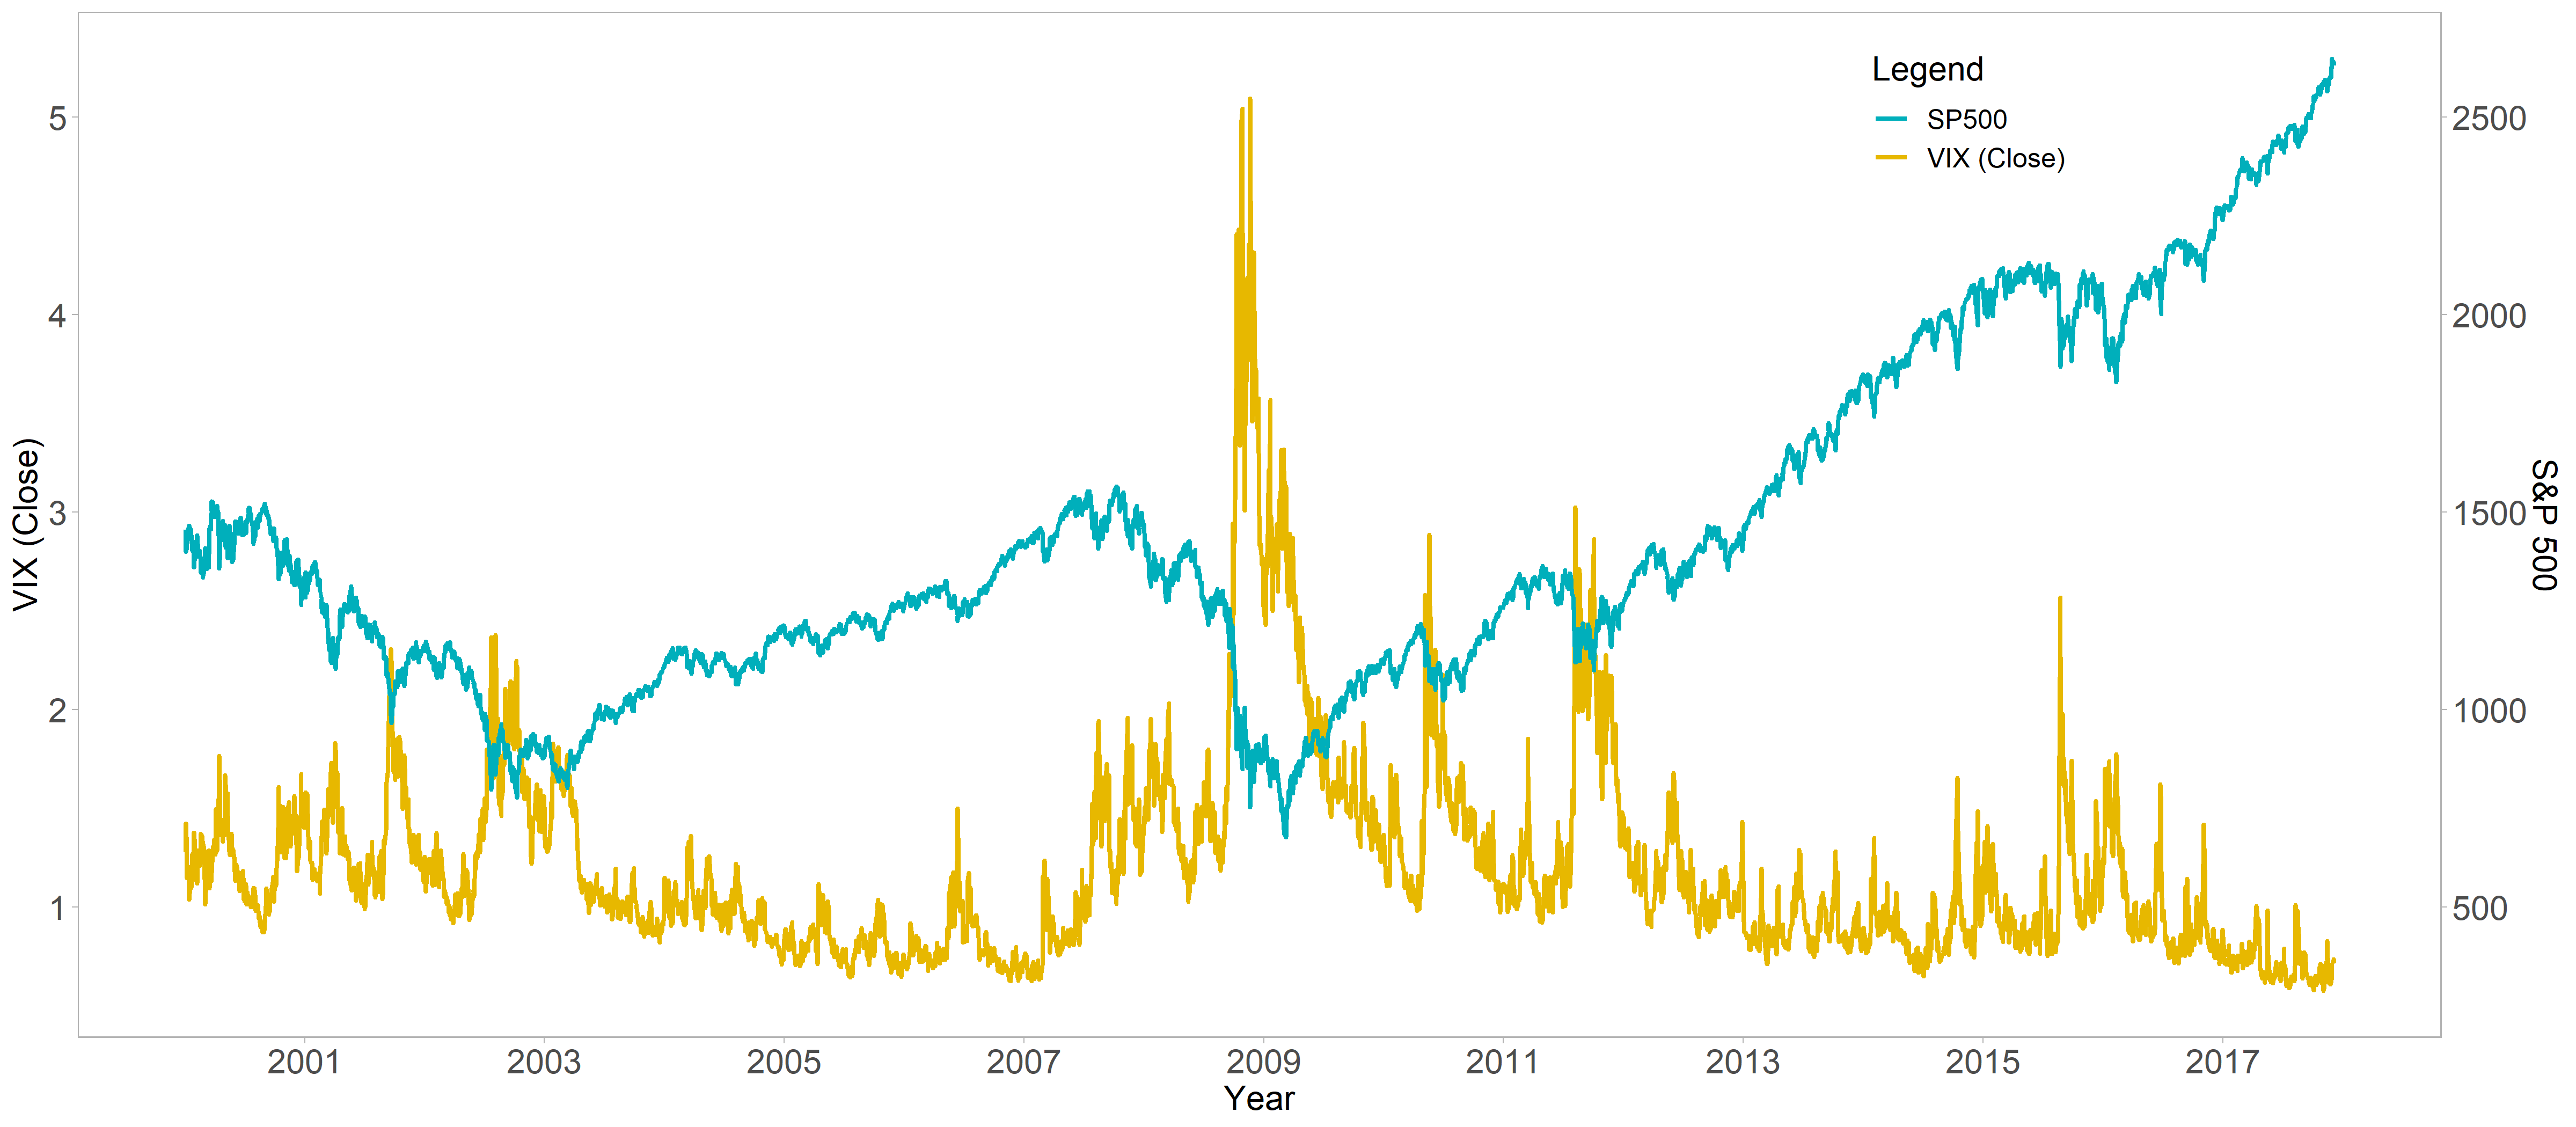
\includegraphics[width=16cm, height=8cm]{pictures/SPandViX.png}
\end{figure}
%
\begin{figure}[!htbp]\label{fig2}\caption{Figure2: \ac{SPX} and RV and VIX}
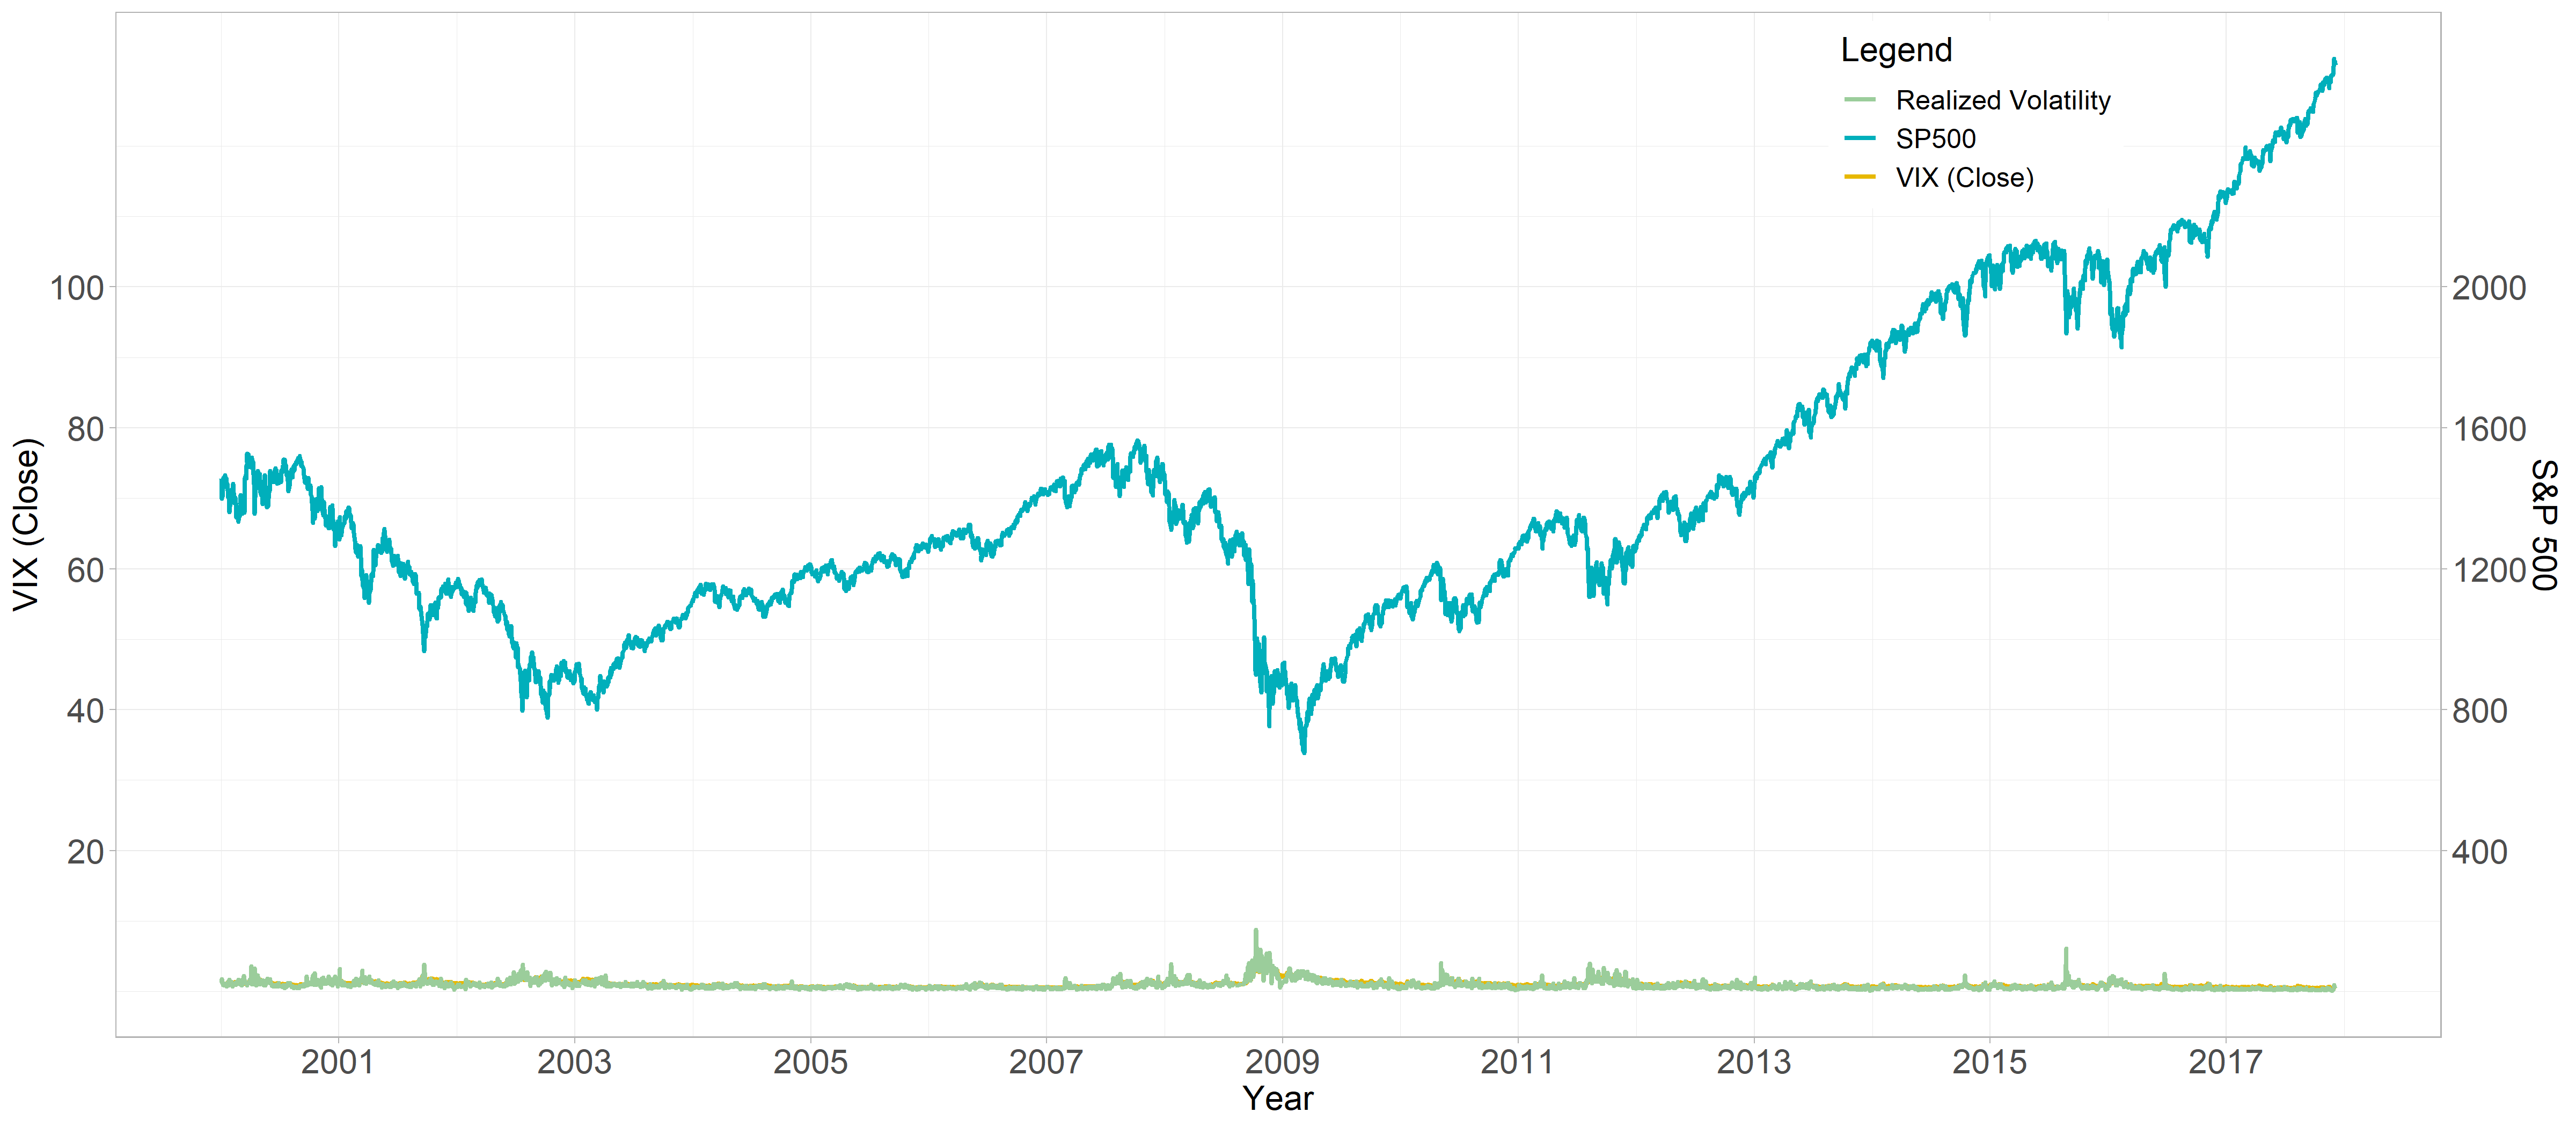
\includegraphics[width=16cm, height=8cm]{pictures/SPandVolandViX.png}
\end{figure}
%

\section{Tables}

% Table created by stargazer v.5.2.2 by Marek Hlavac, Harvard University. E-mail: hlavac at fas.harvard.edu
% Date and time: Fr, Jan 11, 2019 - 17:33:58
\begin{table}[!htbp] \centering 
  \caption{summary statistics: variables} 
  \label{tab:summary1} 
\begin{tabular}{@{\extracolsep{5pt}}lccccccc} 
\\[-1.8ex]\hline 
\hline \\[-1.8ex] 
Statistic & \multicolumn{1}{c}{N} & \multicolumn{1}{c}{Min} & \multicolumn{1}{c}{Max} & \multicolumn{1}{c}{Mean} & \multicolumn{1}{c}{St. Dev.} & \multicolumn{1}{c}{Skewness} & \multicolumn{1}{c}{Kurtosis} \\
\hline \\[-1.8ex] 
\multicolumn{8}{c}{All time periods} \\
\hline \\[-1.8ex] 
RV & 4,434 & 0.110 & 8.802 & 0.874 & 0.615 & 3.127 & 17.751 \\ 
VIX & 4,434 & 0.576 & 5.094 & 1.196 & 0.525 & 2.552 & 9.787 \\ 
Weekly RV & 4,434 & 0.183 & 5.586 & 0.874 & 0.556 & 2.757 & 12.451 \\ 
Monthly RV & 4,434 & 0.223 & 4.375 & 0.876 & 0.512 & 2.534 & 10.051\\ 
Weekly VIX & 4,434 & 0.596 & 4.593 & 1.197 & 0.519 & 2.510 & 9.235 \\ 
Monthly VIX & 4,434 & 0.618 & 4.126 & 1.198 & 0.504 & 2.491 & 8.853 \\ 
\hline \\[-1.8ex] 
\multicolumn{8}{c}{During crisis} \\
\hline \\[-1.8ex] 
RV & 1,252 & 0.213 & 8.802 & 1.171 & 0.834 & 2.713 & 11.399\\ 
VIX  & 1,259 & 0.847 & 5.094 & 1.623 & 0.695  & 1.941 &  4.232\\ 
Weekly RV & 1,259 & 0.257 & 5.586 & 1.169 & 0.753 & 2.409 & 7.417\\ 
Monthly RV & 1,259 & 0.423 & 4.375 & 1.172 & 0.689 & 2.178 & 5.448\\ 
Weekly VIX & 1,259 & 0.885 & 4.593 & 1.623 & 0.684  &  1.885 & 3.753\\ 
Monthly VIX & 1,259 & 0.946 & 4.126 & 1.625 & 0.662 & 1.837 & 3.311\\ 
\hline \\[-1.8ex] 
\multicolumn{8}{c}{Outside of crisis} \\
\hline \\[-1.8ex] 
RV & 3,229 & 0.110 & 6.109 & 0.762 & 0.454 & 2.252 & 10.798\\ 
VIX & 3,251 & 0.576 & 2.566 & 1.034 & 0.307 & 1.206 & 1.365 \\ 
Weekly RV & 3,246 & 0.183 & 3.165 & 0.765 & 0.400 & 1.564 &  3.441\\ 
Monthly RV & 3,229 & 0.223 & 2.367 & 0.764 & 0.363 & 1.308 & 1.687  \\ 
Weekly VIX & 3,246 & 0.596 & 2.188 & 1.034 & 0.300  & 1.157 &  1.047 \\ 
Monthly VIX & 3,229 & 0.618 & 2.014 & 1.033 & 0.285 &  1.1 & 0.78\\ 
\hline \\[-1.8ex] 
\end{tabular} 
\end{table} 

% Table created by stargazer v.5.2.2 by Marek Hlavac, Harvard University. E-mail: hlavac at fas.harvard.edu
% Date and time: Fr, Jan 11, 2019 - 18:36:21
\begin{table}[!htbp] \centering 
  \caption{summary statistics: logarithm variables} 
  \label{tab:summary2} 
\begin{tabular}{@{\extracolsep{5pt}}lccccccc} 
\\[-1.8ex]\hline 
\hline \\[-1.8ex] 
Statistic & \multicolumn{1}{c}{N} & \multicolumn{1}{c}{Min} & \multicolumn{1}{c}{Max} & \multicolumn{1}{c}{Mean} & \multicolumn{1}{c}{St. Dev.} & \multicolumn{1}{c}{Skewness} & \multicolumn{1}{c}{Kurtosis} \\ 
\hline \\[-1.8ex] 
\multicolumn{8}{c}{All time periods} \\
\hline \\[-1.8ex] 
RV & 1,236 & $-$9.664 & 0.777 & $-$1.469 & 1.262 & -1.369 & 3.185 \\ 
VIX & 2,528 & $-$8.005 & 0.487 & $-$1.562 & 1.190 & -1.294 & 2.586\\ 
Weekly RV & 4,434 & 0.183 & 5.586 & 0.874 & 0.556  &  2.757 & 12.451\\ 
Monthly RV & 4,434 & $-$1.501 & 1.476 & $-$0.259 & 0.483 &  0.487 & 0.357  \\ 
Weekly VIX & 4,434 & $-$0.518 & 1.525 & 0.111 & 0.350 & 0.933 &  1.117  \\ 
Monthly VIX & 4,434 & $-$0.481 & 1.417 & 0.115 & 0.340 &  0.963 &   1.227\\ 
\hline \\[-1.8ex] 
\multicolumn{8}{c}{During crisis} \\
\hline \\[-1.8ex] 
RV & 1,252 & 0.213 & 8.802 & 1.171 & 0.834 & 2.713 & 11.399\\ 
VIX & 1,259 & 0.847 & 5.094 & 1.623 & 0.695 & 1.941 & 4.232 \\ 
Weekly RV & 1,259 & 0.257 & 5.586 & 1.169 & 0.753 &  2.409 & 7.417 \\ 
Monthly RV & 1,259 & 0.423 & 4.375 & 1.172 & 0.689 & 2.178 & 5.448\\ 
Weekly VIX & 1,259 & 0.885 & 4.593 & 1.623 & 0.684 &  1.885 &  3.753\\ 
Monthly VIX & 1,259 & 0.946 & 4.126 & 1.625 & 0.662 &  1.837 &  3.311\\ 
\hline \\[-1.8ex] 
\multicolumn{8}{c}{Outside of crisis} \\                           
\hline \\[-1.8ex] 
RV & 3,229 & 0.110 & 6.109 & 0.762 & 0.454 & 2.252  & 10.798\\ 
VIX & 3,251 & 0.576 & 2.566 & 1.034 & 0.307 & 1.206 & 1.365\\ 
Weekly RV & 3,246 & 0.183 & 3.165 & 0.765 & 0.400  &  1.564  & 3.441 \\ 
Monthly RV & 3,229 & 0.223 & 2.367 & 0.764 & 0.363  & 1.308 & 1.687\\ 
Weekly VIX & 3,246 & 0.596 & 2.188 & 1.034 & 0.300  & 1.157 & 1.047\\ 
Monthly VIX & 3,229 & 0.618 & 2.014 & 1.033 & 0.285 & 1.100 & 0.780 \\ 
\hline \\[-1.8ex] 
\end{tabular} 
\end{table} 

\newgeometry{left=1cm,bottom=0.1cm}

% Table created by stargazer v.5.2.2 by Marek Hlavac, Harvard University. E-mail: hlavac at fas.harvard.edu
% Date and time: Sa, Jan 12, 2019 - 09:20:14
\begin{table}[!htbp] \centering 
  \caption{correlation table} 
  \label{tab: correlation} 
\begin{tabular}{@{\extracolsep{5pt}} ccccccccc} 
\\[-1.8ex]\hline 
\hline \\[-1.8ex] 
 & RV & VIX & Daily RV & Weekly RV & Monthly RV & D. VIX & W.VIX & M. VIX \\ 
\hline \\[-1.8ex] 
RV & $1$ & $0.837$ & $0.806$ & $0.823$ & $0.769$ & $0.819$ & $0.781$ & $0.698$ \\ 
VIX & $0.837$ & $1$ & $0.822$ & $0.883$ & $0.903$ & $0.981$ & $0.969$ & $0.926$ \\ 
Daily RV & $0.806$ & $0.822$ & $1$ & $0.890$ & $0.794$ & $0.837$ & $0.803$ & $0.710$ \\ 
Weekly RV & $0.823$ & $0.883$ & $0.890$ & $1$ & $0.903$ & $0.896$ & $0.906$ & $0.809$ \\ 
Monthly RV & $0.769$ & $0.903$ & $0.794$ & $0.903$ & $1$ & $0.910$ & $0.932$ & $0.931$ \\ 
Daily VIX & $0.819$ & $0.981$ & $0.837$ & $0.896$ & $0.910$ & $1$ & $0.982$ & $0.935$ \\ 
Weekly VIX & $0.781$ & $0.969$ & $0.803$ & $0.906$ & $0.932$ & $0.982$ & $1$ & $0.961$ \\ 
Monthly VIX & $0.698$ & $0.926$ & $0.710$ & $0.809$ & $0.931$ & $0.935$ & $0.961$ & $1$ \\ 
\hline \\[-1.8ex] 
\end{tabular} 
\end{table} 

\restoregeometry


\section{Additional Regression Results and Robustness Checks}


% Table created by stargazer v.5.2.2 by Marek Hlavac, Harvard University. E-mail: hlavac at fas.harvard.edu
% Date and time: Sa, Jan 19, 2019 - 20:40:21
\begin{table}[!htbp] \centering 
  \caption{Level regression (whole sample)} 
  \label{newey1} 
\begin{tabular}{@{\extracolsep{5pt}}lccc} 
\\[-1.8ex]\hline 
\hline \\[-1.8ex] 
 & \multicolumn{3}{c}{\textit{Dependent variable:}} \\ 
\cline{2-4} 
\\[-1.8ex] & \multicolumn{3}{c}{Realized Volatility} \\ 
 & Reg1a & Reg2a & Reg3a \\ 
\\[-1.8ex] & (1) & (2) & (3)\\ 
\hline \\[-1.8ex] 
 Intercept & 0.045$^{***}$ & $-$0.324$^{***}$ & $-$0.169$^{***}$ \\ 
  & (0.015) & (0.059) & (0.034) \\ 
  & & & \\ 
 $RV^{(d)}_{t}$ & 0.362$^{***}$ &  & 0.256$^{***}$ \\ 
  & (0.038) &  & (0.040) \\ 
  & & & \\ 
 $RV^{(w)}_{t}$ & 0.391$^{***}$ &  & 0.286$^{***}$ \\ 
  & (0.056) &  & (0.064) \\ 
  & & & \\ 
 $RV^{(m)}_{t}$ & 0.188$^{***}$ &  & $-$0.106$^{**}$ \\ 
  & (0.036) &  & (0.050) \\ 
  & & & \\ 
 $crisis$ & 0.025$^{*}$ & $-$0.214$^{***}$ & $-$0.112$^{***}$ \\ 
  & (0.013) & (0.035) & (0.021) \\ 
  & & & \\ 
 $VIX_{t}$ &  & 1.052$^{***}$ & 0.579$^{***}$ \\ 
  &  & (0.059) & (0.064) \\ 
  & & & \\ 
\hline \\[-1.8ex] 
AIC & 2817.4 & 3104.2 & 2446 \\ 
Observations & 4,434 & 4,434 & 4,434 \\ 
R$^{2}$ & 0.708 & 0.689 & 0.732 \\ 
Adjusted R$^{2}$ & 0.708 & 0.688 & 0.732 \\ 
Residual Std. Error & 0.332 (df = 4429) & 0.343 (df = 4431) & 0.319 (df = 4428) \\ 
\hline 
\hline \\[-1.8ex] 
\textit{Note:}  & \multicolumn{3}{r}{$^{*}$p$<$0.1; $^{**}$p$<$0.05; $^{***}$p$<$0.01} \\ 
\end{tabular} 
\end{table} 
\label{tab:newey1}


% Table created by stargazer v.5.2.2 by Marek Hlavac, Harvard University. E-mail: hlavac at fas.harvard.edu
% Date and time: Di, Jan 15, 2019 - 16:19:13
\begin{table}[!htbp] \centering 
\begin{threeparttable}
  \caption{Level regression} 
  \label{tab:overlap1} 
\begin{tabular}{@{\extracolsep{5pt}}lccc} 
\\[-1.8ex]\hline 
\hline \\[-1.8ex] 
 & \multicolumn{3}{c}{\textit{Dependent variable:}} \\ 
\cline{2-4} 
\\[-1.8ex] & \multicolumn{3}{c}{Realized Volatility} \\ 
 & Reg1a & Reg2a & Reg3a \\ 
\\[-1.8ex] & (1) & (2) & (3)\\ 
\hline \\[-1.8ex] 
 Intercept & 0.046 & $-$0.342$^{***}$ & $-$0.134$^{**}$ \\ 
  & (0.031) & (0.091) & (0.052) \\ 
  & & & \\ 
 $RV^{d}_{t}$ & 0.408$^{***}$ &  & 0.330$^{***}$ \\ 
  & (0.109) &  & (0.116) \\ 
  & & & \\ 
 $RV^{w}_{t}$ & 0.501$^{***}$ &  & 0.394$^{***}$ \\ 
  & (0.126) &  & (0.128) \\ 
  & & & \\ 
 $RV^{m}_{t}$ & 0.072 &  & $-$0.132 \\ 
  & (0.079) &  & (0.083) \\ 
  & & & \\ 
 $crisis$ & $-$0.022 & $-$0.257$^{***}$ & $-$0.131$^{***}$ \\ 
  & (0.029) & (0.058) & (0.035) \\ 
  & & & \\ 
 $VIX_{t}$ &  & 1.092$^{***}$ & 0.460$^{***}$ \\ 
  &  & (0.094) & (0.089) \\ 
  & & & \\ 
\hline \\[-1.8ex] 
AIC & 192.5 & 281.8 & 166 \\ 
Observations & 456 & 456 & 456 \\ 
R$^{2}$ & 0.757 & 0.701 & 0.771 \\ 
Adjusted R$^{2}$ & 0.754 & 0.700 & 0.769 \\ 
Residual Std. Error & 0.297 (df = 451) & 0.328 (df = 453) & 0.288 (df = 450) \\ 
\hline 
\hline \\[-1.8ex] 
\textit{Note:}  & \multicolumn{3}{r}{$^{*}$p$<$0.1; $^{**}$p$<$0.05; $^{***}$p$<$0.01} \\ 
\end{tabular} 
 \begin{tablenotes}
      \small
      \item The numbers in the brackets are the standard errors of the parameters computed with Newey-West covariance correction, which are robust to autocorrelated and heteroscedastic error terms, see \textcite{newey1987}.
    \end{tablenotes}
  \end{threeparttable}
\end{table} 
\label{tab:overlap1}
%

% Table created by stargazer v.5.2.2 by Marek Hlavac, Harvard University. E-mail: hlavac at fas.harvard.edu
% Date and time: So, Jan 13, 2019 - 10:25:28
\begin{table}[!htbp] \centering 
  \caption{logarithmic regression} 
  \label{} 
\begin{tabular}{@{\extracolsep{5pt}}lccc} 
\\[-1.8ex]\hline 
\hline \\[-1.8ex] 
 & \multicolumn{3}{c}{\textit{Dependent variable:}} \\ 
\cline{2-4} 
\\[-1.8ex] & \multicolumn{3}{c}{Realized Volatility} \\ 
 & Reg1b & Reg2b & Reg3b \\ 
\\[-1.8ex] & (1) & (2) & (3)\\ 
\hline \\[-1.8ex] 
 c & $-$0.001 & $-$0.364$^{***}$ & $-$0.049$^{*}$ \\ 
  & (0.018) & (0.026) & (0.028) \\ 
  & & & \\ 
 $ ln(RV^{d}_{t})$ & 0.346$^{***}$ &  & 0.352$^{***}$ \\ 
  & (0.064) &  & (0.064) \\ 
  & & & \\ 
 $ln(RV^{w}_{t})$ & 0.408$^{***}$ &  & 0.432$^{***}$ \\ 
  & (0.078) &  & (0.080) \\ 
  & & & \\ 
 $ ln(RV^{m}_{t})$ & 0.171$^{***}$ &  & 0.003 \\ 
  & (0.054) &  & (0.088) \\ 
  & & & \\ 
 $crisis$ & $-$0.017 & $-$0.169$^{***}$ & $-$0.063$^{*}$ \\ 
  & (0.027) & (0.062) & (0.034) \\ 
  & & & \\ 
 $ln(VIX_{t})$ &  & 1.229$^{***}$ & 0.236$^{**}$ \\ 
  &  & (0.074) & (0.104) \\ 
  & & & \\ 
\hline \\[-1.8ex] 
AIC & 126.4 & 415.1 & 123.9 \\ 
Observations & 456 & 455 & 455 \\ 
R$^{2}$ & 0.748 & 0.522 & 0.751 \\ 
Adjusted R$^{2}$ & 0.746 & 0.519 & 0.748 \\ 
Residual Std. Error & 0.276 (df = 451) & 0.380 (df = 452) & 0.275 (df = 449) \\ 
\hline 
\hline \\[-1.8ex] 
\textit{Note:}  & \multicolumn{3}{r}{$^{*}$p$<$0.1; $^{**}$p$<$0.05; $^{***}$p$<$0.01} \\ 
\end{tabular} 
\end{table} 
\label{tab:overlap2}
%


	 % die entsprechenden Teile müssen ebenfalls im entsprechenden Ordner vorhanden sein. Jeder Teil muss mit dem Magic Comment %!TEX root = ../Main.tex  beginnen

	\newpage
	\pagenumbering{Roman}
	\printbibliography


\section{Eidesstattliche Erklärung zur Hausarbeit}

Ich erkläre hiermit ehrenwörtlich, dass ich die vorliegende Seminararbeit / Bachelorarbeit/  Masterarbeit mit dem Thema
\vspace{1cm}

\begin{center}
Thema der Arbeit
\end{center}
\vspace{1cm}

\noindent selbstständig und ohne fremde Hilfe angefertigt habe.

\vspace{1cm}
\noindent Die Übernahme wörtlicher Zitate sowie die Verwendung der Gedanken anderer Autoren habe ich an den entsprechenden Stellen der Arbeit kenntlich gemacht.

\vspace{1cm}
\noindent Ich bin mir bewusst, dass eine falsche Erklärung rechtliche Folgen haben wird.

\vspace{3cm}


\begin{tabulary}{\textwidth}{Lp{2in}@{}}
& \hrulefill \\
Ort, den \today& Name \\
\end{tabulary}
\end{document}
